\documentclass[dissertation.tex]{subfiles} 
\begin{document}

\chapter{Data Analysis}
\label{chap:Data Analysis}

%make sure all plots have bold font removed are are marked as either data or simulation

The signature of GGM SUSY particle production in this search is an excess of two-photon events with high \MET.  \MET is reconstructed using the particle flow algorithm as described in Sec.~\ref{sec:MET}.  Candidate two-photon events, as well as control events, are selected according to the offline object criteria presented in Secs.~\ref{sec:Photons} and~\ref{sec:Electrons}, the event quality criteria in Sec.~\ref{sec:Event Quality}, and the trigger requirements in Sec.~\ref{sec:HLT}.  These are summarized in Table~\ref{tab:selection_summary}.

\begin{table}[hcbp]
\caption{Selection criteria for $\gamma\gamma$, $e\gamma$, $ee$, and $\mathit{ff}$ events.}
\centering
\begin{tabular}{|c|c|c|c|c|}
\hline
\multirow{2}{*}{Variable} & \multicolumn{4}{c|}{Cut} \\
\cline{2-5}
& $\gamma\gamma$ & $e\gamma$ & $ee$ & $\mathit{ff}$ \\
\hline
\hline
%HLT & \begin{tabular}[c]{@{}c@{}}26IsoVL/\\18\\\\36CaloIdL/\\22CaloIdL\\\\36CaloIdLIsoVL/\\22CaloIdLIsoVL\end{tabular} & \begin{tabular}[c]{@{}c@{}}26IsoVL/\\18\\\\36CaloIdL/\\22CaloIdL\\\\36CaloIdLIsoVL/\\22CaloIdLIsoVL\end{tabular} & \begin{tabular}[c]{@{}c@{}}26IsoVL/\\18\\\\36CaloIdL/\\22CaloIdL\\\\36CaloIdLIsoVL/\\22CaloIdLIsoVL\end{tabular} & \begin{tabular}[c]{@{}c@{}}26IsoVL/\\18\\\\36CaloIdL/\\22CaloIdL\\\\36CaloIdLIsoVL/\\22CaloIdLIsoVL\\\\36CaloIdLIsoVL/\\22R9Id\\\\36R9Id/\\22CaloIdLIsoVL\\\\36R9Id/\\22R9Id\end{tabular} \\
%\hline
HLT match & IsoVL & IsoVL & IsoVL & IsoVL $||$ R9Id \\
\hline
$E_{T}$ & \begin{tabular}[c]{@{}c@{}}$> 40$/\\$> 25$ GeV\end{tabular} & \begin{tabular}[c]{@{}c@{}}$> 40$/\\$> 25$ GeV\end{tabular} & \begin{tabular}[c]{@{}c@{}}$> 40$/\\$> 25$ GeV\end{tabular} & \begin{tabular}[c]{@{}c@{}}$> 40$/\\$> 25$ GeV\end{tabular} \\
\hline
SC $|\eta|$ & $< 1.4442$ & $<1.4442$ & $< 1.4442$ & $<1.4442$ \\
\hline
$H/E$ & $<0.05$ & $<0.05$ & $<0.05$ & $<0.05$ \\
\hline
$R9$ & $< 1$ & $< 1$ & $< 1$ & $< 1$ \\
\hline
Pixel seed & No/No & Yes/No & Yes/Yes & No/No \\
\hline
$I_{\mathrm{comb}}$, $\sigma_{i\eta i\eta}$ & \begin{tabular}[c]{@{}c@{}}$< 6$ GeV \&\&\\$< 0.011$\end{tabular} & \begin{tabular}[c]{@{}c@{}}$< 6$ GeV \&\&\\$< 0.011$\end{tabular} & \begin{tabular}[c]{@{}c@{}}$< 6$ GeV \&\&\\$< 0.011$\end{tabular} & \begin{tabular}[c]{@{}c@{}}$< 20$ GeV \&\&\\($\geq 6$ GeV $||$\\$\geq 0.011$)\end{tabular} \\
\hline
JSON & Yes & Yes & Yes & Yes \\
\hline
No. good PVs & $\geq 1$ & $\geq 1$ & $\geq 1$ & $\geq 1$ \\
\hline
$\Delta R_{\mathrm{EM}}$ & $> 0.6$ & $> 0.6$ & $> 0.6$ & $> 0.6$ \\
\hline
$\Delta\phi_{\mathrm{EM}}$ & $\geq 0.05$ & $\geq 0.05$ & $\geq 0.05$ & $\geq 0.05$ \\
\hline
\end{tabular}
\label{tab:selection_summary}
\end{table}

This search utilizes 4.7 $\mbox{fb}^{-1}$ of CMS data collected during the period April-December 2011, corresponding to the following datasets \cite{DAS}:

\begin{itemize}
\item \verb+/Photon/Run2011A-05Jul2011ReReco-ECAL-v1/AOD+
\item \verb+/Photon/Run2011A-05Aug2011-v1/AOD+
\item \verb+/Photon/Run2011A-03Oct2011-v1/AOD+
\item \verb+/Photon/Run2011B-PromptReco-v1/AOD+
\end{itemize}

The search strategy is to model the backgrounds to the GGM SUSY signal using \MET shape templates derived from the control samples, and then to look for a high-\MET excess above the estimated background in the $\gamma\gamma$ sample.  There are two categories of backgrounds: QCD processes with no real \MET and electroweak processes with real \MET from neutrinos.  The relevant QCD background processes are multijet production with at least two jets faking photons, photon + jet production with at least one jet faking a photon, diphoton production, and $Z$ production with a radiated photon where at least one of the $Z$ decay products (typically a jet) fakes a photon.  The relevant electroweak background processes, which are small compared to the QCD background, involve $W\rightarrow e\nu$ decay with a recoiling jet that fakes a photon or a real radiated photon.  In both cases, the electron is misidentified as a photon due to a small inefficiency in reconstructing the electron pixel seed.  The main diagrams contributing to the QCD(electroweak) backgrounds are shown in Figure~\ref{fig:QCD_background_diagrams}(\ref{fig:EW_background_diagrams}).  \textcolor{red}{\textbf{Generate these Feynman diagrams.}}

%QCD EM-enriched (isub=11,12,13,28,53,68) (mstp82=4 ==> multiple int. assuming varying impact parameter and hadronic overlap consistent with a double gaussian matter distribution, but turning off at low pt)
%q_i q_j --> q_i q_j
%q_i q_i --> q_j q_j
%q_i q_i_bar --> g g
%q_i g --> q_i g
%g g --> q_i q_i_bar
%g g --> g g
%photon + jet EM enriched (isub=14,18,29)
%q_i q_i_bar --> g gamma
%q_i q_i_bar --> gamma gamma
%q_i g --> q_i gamma
%diphoton + jets (pp-->gammagamma, +1 j, +2 j (j ==> sum over gluons and light quarks, not t/b)), tree level to order X (QCD) and Y (QED)
%DiPhotonBorn: q_i q_i_bar --> gamma gamma
%DiPhotonBox:  g g --> gamma gamma
%W + jets
%W + photon
%Z + photon
%

%Wgg, Zgg (negligible)

%\begin{figure}
%	\centering
%	\subfloat[Dijet production via $gg$ and $qg$ interactions.]{\label{fig:dijet}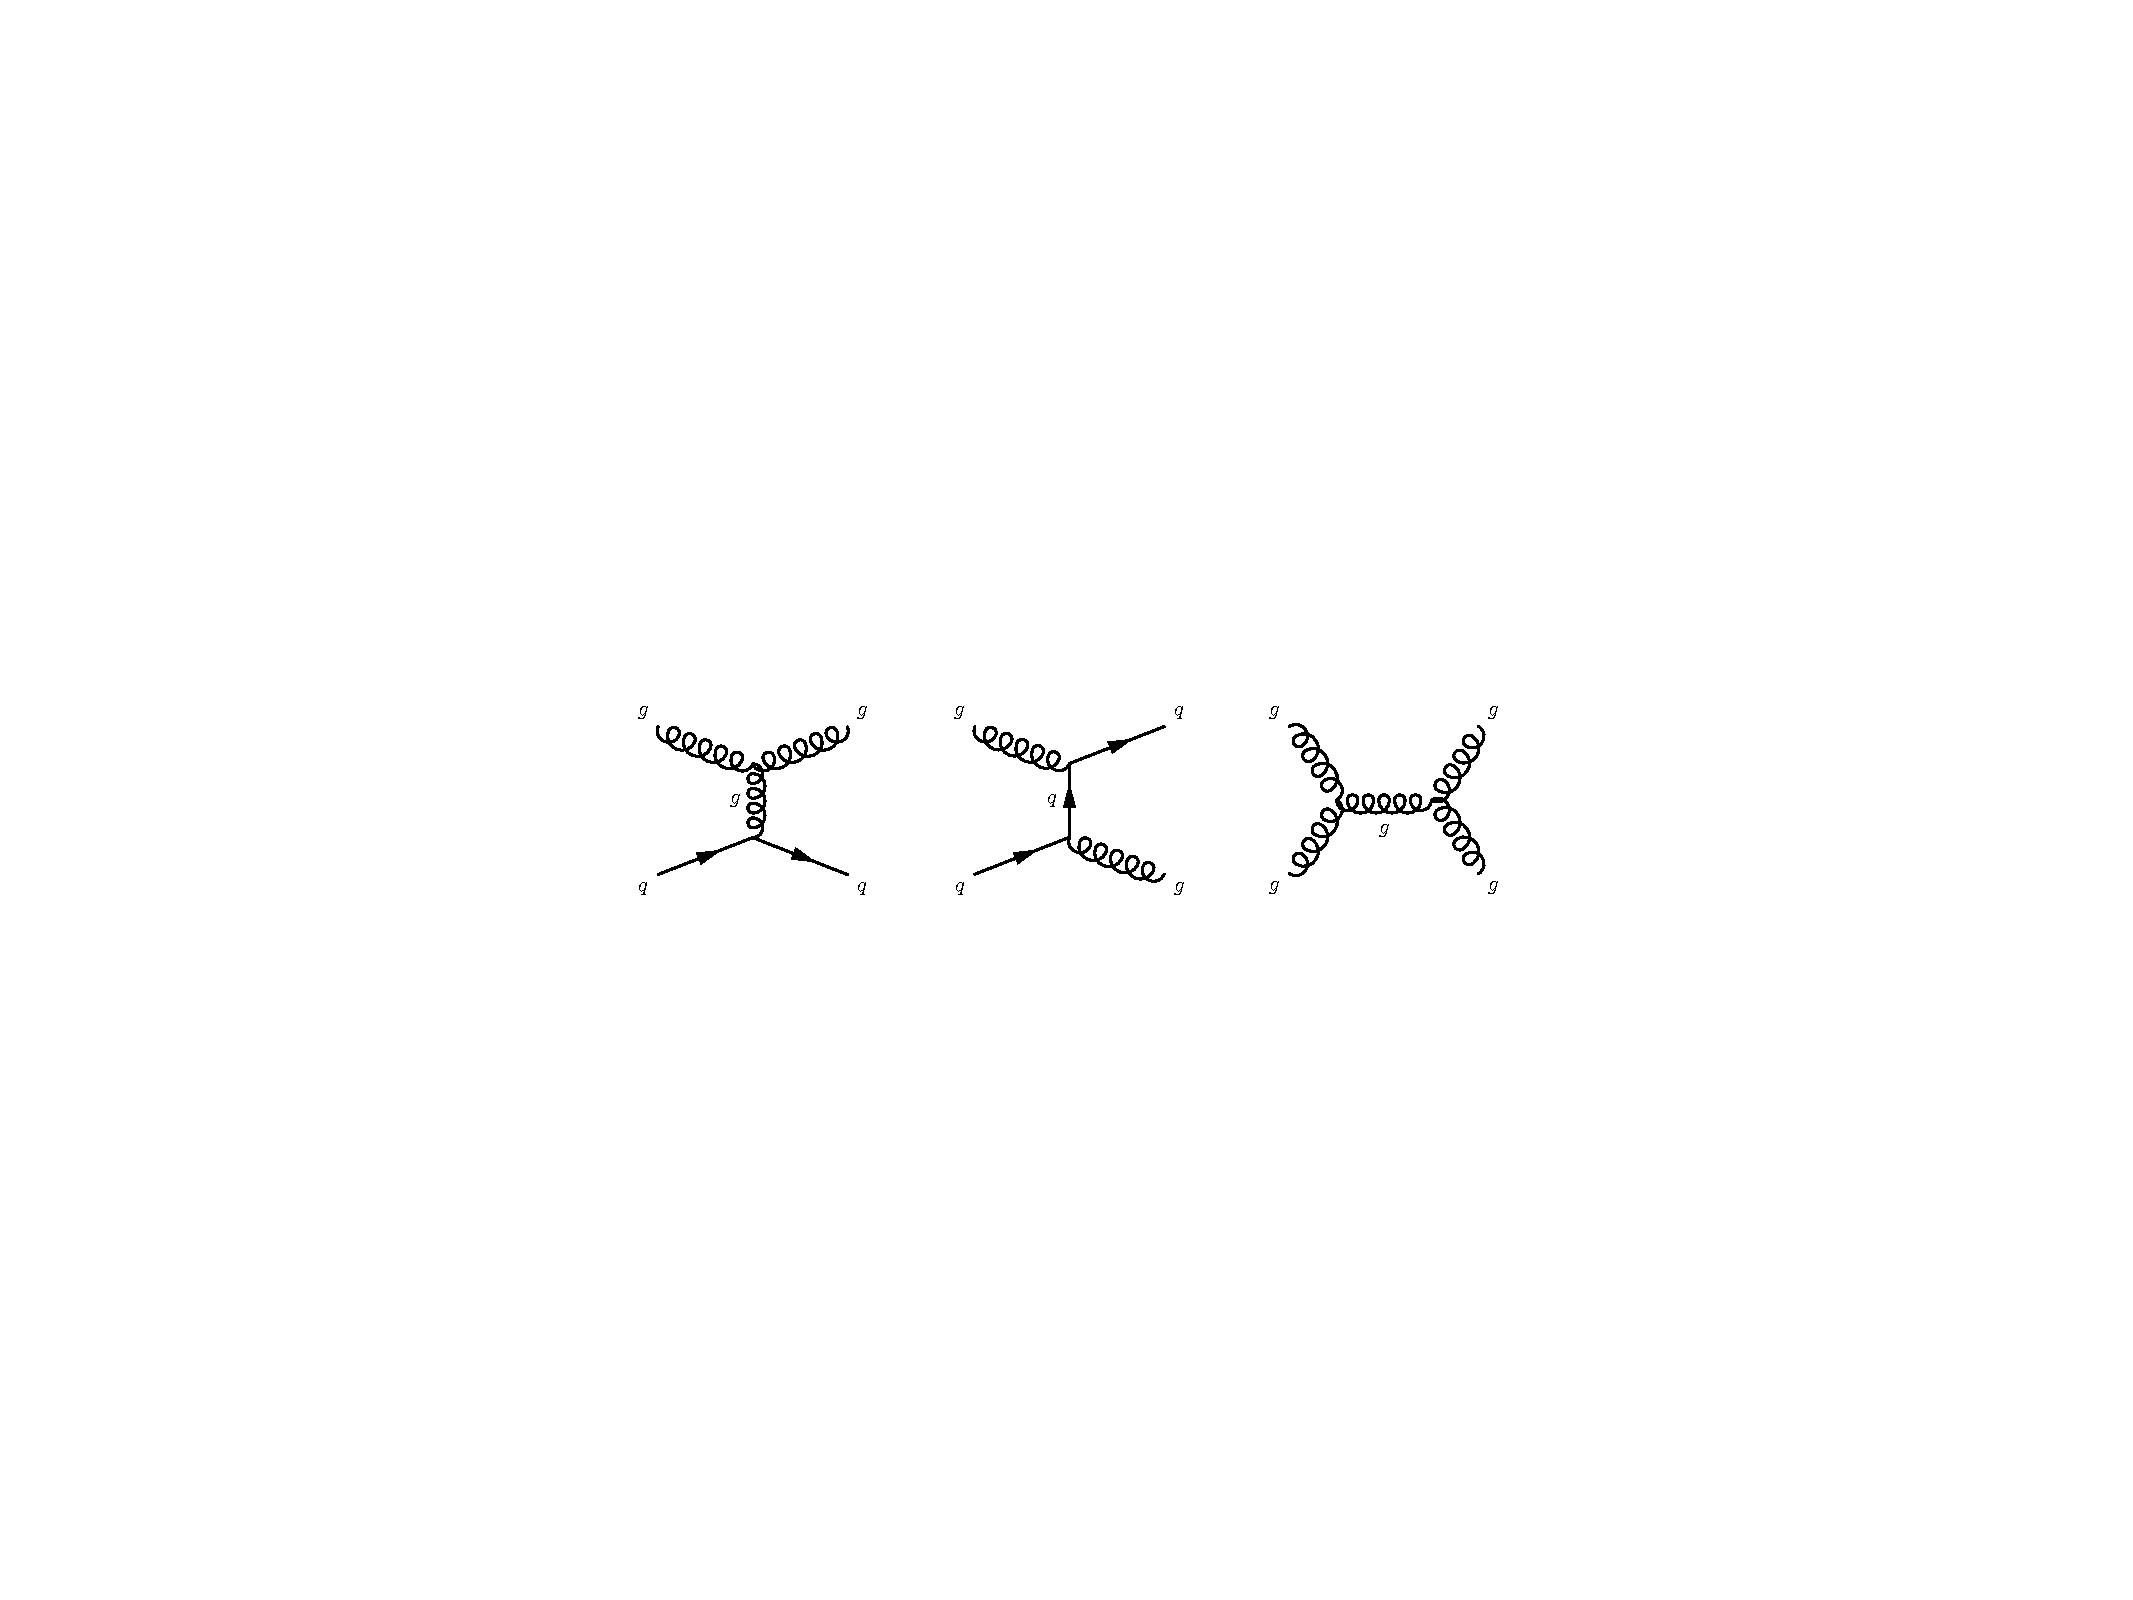
\includegraphics[scale=1.35]{dijet}}
%	\hspace{1cm}
%	\subfloat[Photon + jet production via $qg$ interactions.]{\label{fig:photon_jet}\includegraphics[scale=1.35]{photon_jet}}
%	\\
%	\subfloat[Diphoton production via $q\bar{q}$ and $gg$ interactions.]{\label{fig:diphoton}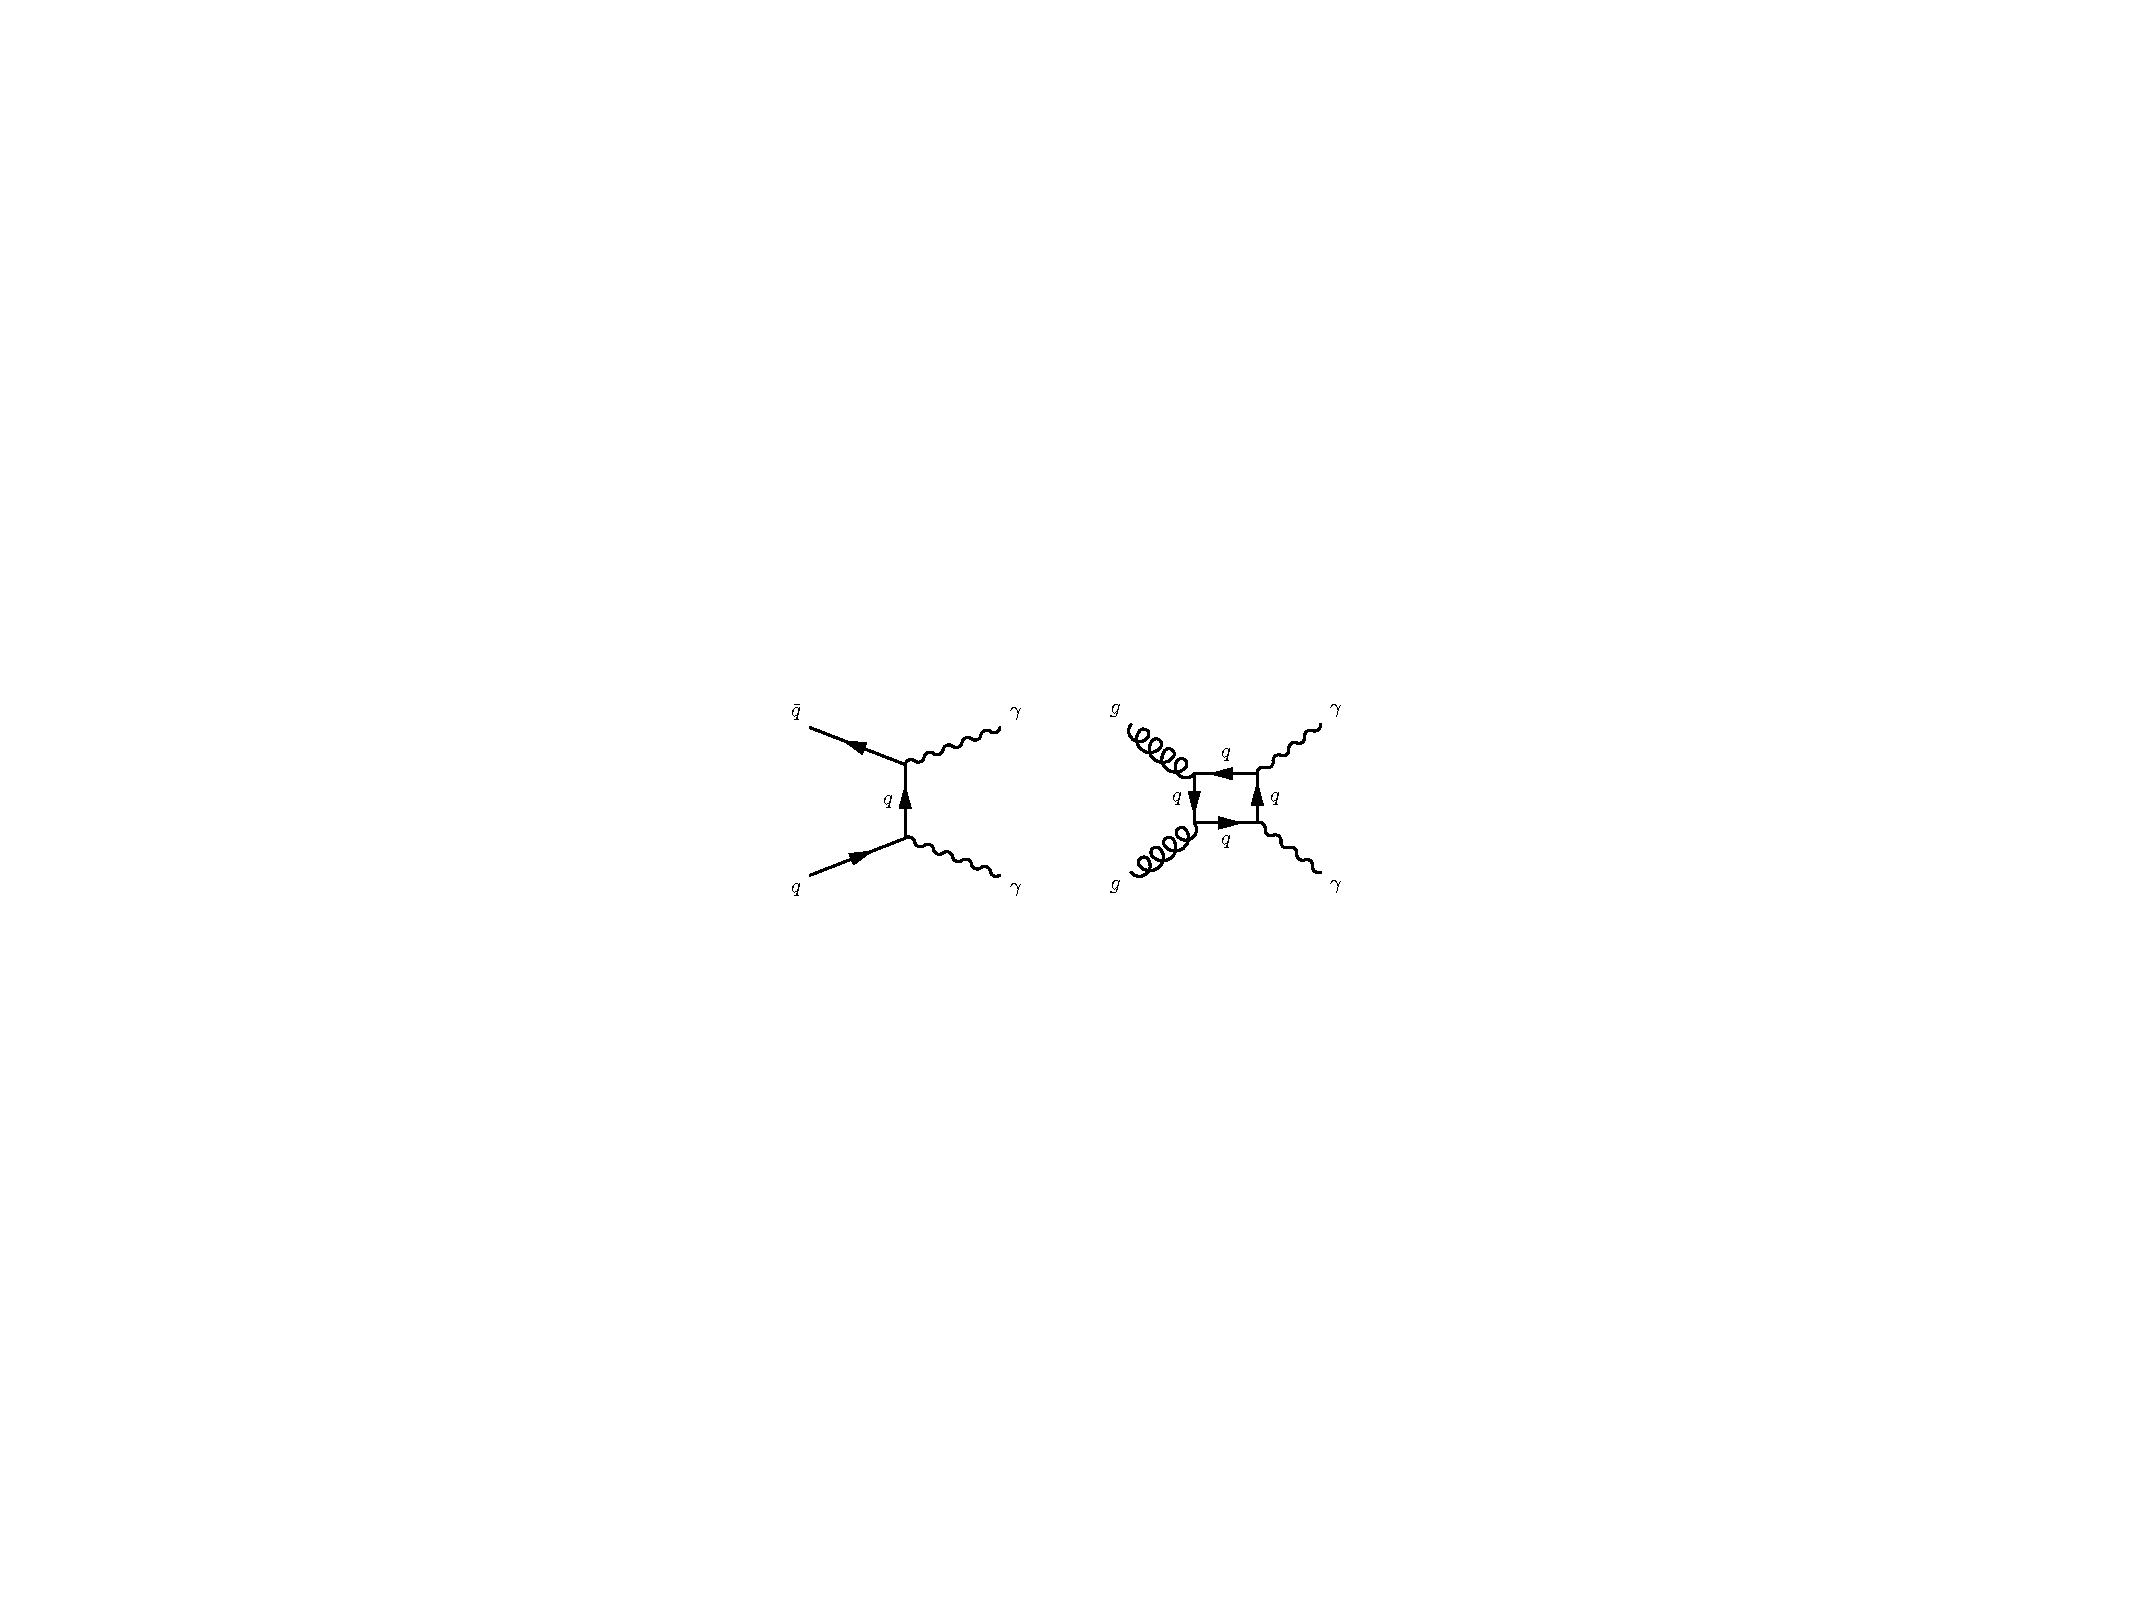
\includegraphics[scale=1.8]{diphoton}}
%	\hspace{1cm}
%	\subfloat[$Z\gamma$ production.]{\label{fig:Zgamma}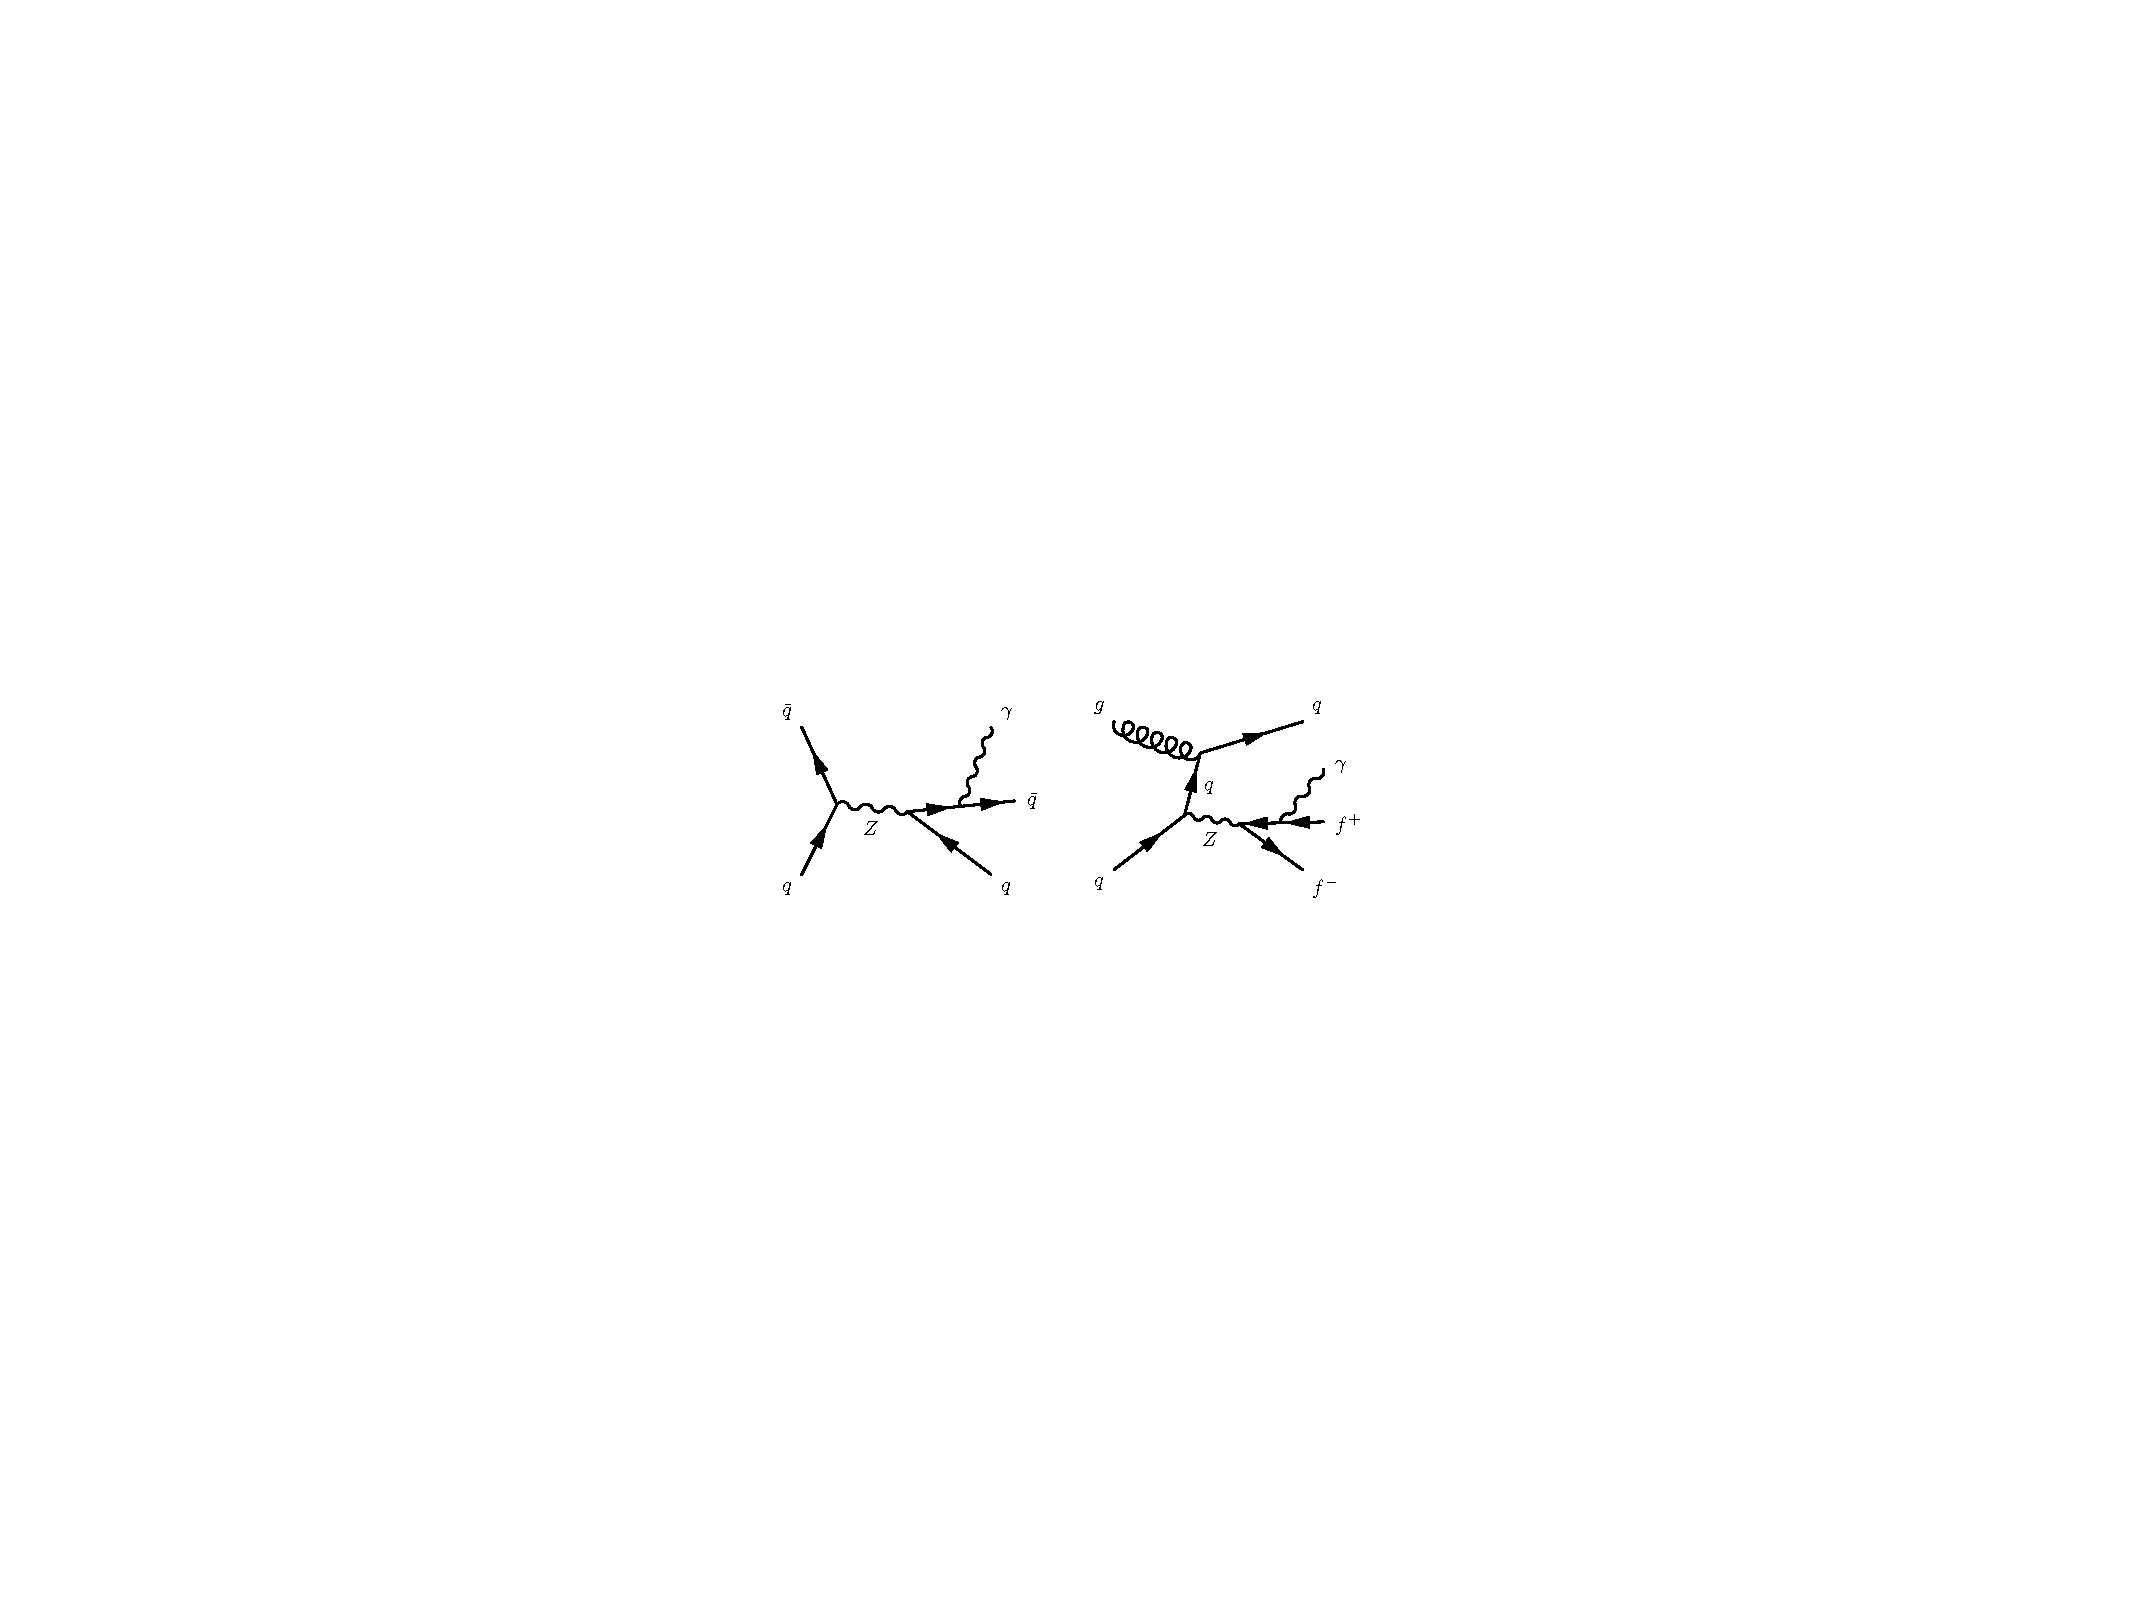
\includegraphics[scale=1.8]{Zgamma}}
%	\caption{Representative Feynman diagrams of some QCD backgrounds to the GGM SUSY search with instrumental effects described.}
%	\label{fig:QCD_background_diagrams}
%\end{figure}
%
%\begin{figure}
%	\centering
%	\subfloat[$W\gamma$ production.]{\label{fig:Wgamma}\includegraphics[scale=1.35]{Wgamma}}
%	\hspace{1cm}
%	\subfloat[$W$ + jet production.]{\label{fig:W_jet}\includegraphics[scale=1.35]{W_jet}}
%	\caption{Representative Feynman diagrams of some electoweak backgrounds to the GGM SUSY search with instrumental effects described.}
%	\label{fig:EW_background_diagrams}
%\end{figure}

Figure~\ref{fig:MET_data_vs_MC_backgrounds} shows the \MET spectrum of the $\gamma\gamma$ search data sample overlaid on the \MET spectra of MC simulated background components.  The MC spectra are normalized to the integrated luminosity of the $\gamma\gamma$ data sample.  \textcolor{red}{\textbf{Make this plot.}}  The dominant background components are QCD inclusive photon processes.  The MC is not used in the actual background estimation.  It is just shown here to illustrate the breakdown of backgrounds.

%\begin{figure}
%	\centering
%	\includegraphics[scale=1.35]{MET_data_vs_MC_backgrounds}
%	\caption{\MET spectrum of the $\gamma\gamma$ search data sample overlaid on the \MET spectra of MC simulated background components.  The MC spectra are normalized to the integrated luminosity of the $\gamma\gamma$ data sample.  A description of the MC samples used may be found in Appendix~\ref{chap:Monte Carlo Samples}}.
%	\label{fig:MET_data_vs_MC_backgrounds}
%\end{figure}

Data control samples are used to model all of the backgrounds.  The primary control sample used to model the QCD background is the $\mathit{ff}$ sample, which is similar to the candidate $\gamma\gamma$ sample but with combined isolation or $\sigma_{i\eta i\eta}$ cuts inverted.  The cuts on these variables are used to distinguish between photons and jets, so by inverting those cuts, the resulting $\mathit{ff}$ sample becomes enriched with QCD dijets.  Because the fake photons are still required to pass a tight cut on $H/E$, they are guaranteed to be very electromagnetic jets, with an EM energy scale and resolution similar to that of the candidate photons.  This insures that the resulting estimate of the \MET shape does not have too long of a tail from severe HCAL mis-measurements that are actually rare in the $\gamma\gamma$ sample, as shown in Figure~\ref{fig:MET_MC_ggVsFF_varyHOverE}.  \textcolor{red}{\textbf{Plot the $\gamma\gamma$/$\mathit{ff}$ \MET agreement for different values of the ff $H/E$ cut in MC.  Make the same plot in data for a restricted \MET range?}}

%\begin{figure}
%	\centering
%	\subfloat[MC.  See App.~\ref{chap:Monte Carlo Samples} for the MC samples used.]{\label{fig:MET_MC_ggVsFF_varyHOverE_MC}\includegraphics[scale=1.35]{MET_MC_ggVsFF_varyHOverE_MC}}
%	\hspace{1cm}
%	\subfloat[Data, restricted to $\MET < 100$ GeV.]{\label{fig:MET_MC_ggVsFF_varyHOverE_data}\includegraphics[scale=1.35]{MET_MC_ggVsFF_varyHOverE_data}}
%	\caption{\MET spectra of the $\gamma\gamma$ and $\mathit{ff}$ samples for various values of the $\mathit{ff} H/E$ cut.}
%	\label{fig:MET_MC_ggVsFF_varyHOverE}
%\end{figure}

As a cross-check, the $ee$ sample is also used to model the QCD background.  This sample of $Z$ decays should have no true \MET, just like the $\mathit{ff}$ sample, and the electron definition (differing from the photon definition only in the presence of a pixel seed) insures that the electron energy scale and resolution is similar to that of the photon.

Finally, the $e\gamma$ sample is used to model the electroweak background from $W\rightarrow e\nu$ decays.  The $e\gamma$ \MET distribution is scaled by the electron$\rightarrow$photon misidentification rate to predict the number of $W\gamma$ and $W$ + jet events in the $\gamma\gamma$ sample.

The remainder of this chapter describes the data analysis procedures and the final results of the search.  Sec.~\ref{sec:Modeling the QCD Background} addresses the QCD background estimation.  Sec.~\ref{sec:Modeling the Electroweak background} addresses the electroweak background estimation.  The chapter concludes with a discussion of systematic errors in Sec.~\ref{sec:Systematic Errors} and a presentation of the final results in Sec.~\ref{sec:Results}.

\section{Modeling the QCD Background}
\label{sec:Modeling the QCD Background}

\subsection{Outline of the Procedure}
\label{sec:Outline of the Procedure}

Due to the fact that the CMS ECAL energy resolution is much better than the HCAL energy resolution, the energies of the two candidate photons in the events of the $\gamma\gamma$ sample are typically measured to far greater accuracy and precision than the energy of the hadronic recoil in those events.  Therefore, fake \MET in the $\gamma\gamma$ sample is almost entirely the result of hadronic mis-measurement in QCD dijet, photon + jet, and diphoton events.  The strategy employed to model this background is to find a control sample in data consisting of two well-measured EM objects, just like the candidate $\gamma\gamma$ sample, and assign each event a weight to account for the underlying kinematic differences between the control and candidate samples.  Once the reweighted \MET spectrum of the control sample is created, it is then normalized in the low-\MET region, the assumption being that GGM SUSY does not predict a significant amount of events at low \MET.  There are three aspects to this QCD background estimation procedure that bear highlighting:

\begin{description}
\item[Choice of control sample] Since the underlying cause of \MET in the candidate sample is mis-measured hadronic activity, a control sample with similar hadronic activity to the candidate sample should be chosen.  Hadronic activity refers to number of jets, jet $E_{T}$, pileup, etc.
\item[Reweighting] The control sample is reweighted so that its \MET spectrum appears as it would if the control sample had the same kinematic properties as the candidate sample (i.e. particle $p_{T}$ and $\eta$ distributions, etc.).  By choosing an appropriate control sample and reweighting it, the control \MET distribution should now match both the hadronic activity and the kinematics of the candidate sample.
\item[Normalization] Finally, the control \MET distribution is normalized in a region of low \MET, where contamination from the expected GGM SUSY signal is small.  This implies an extrapolation of the low-\MET QCD background prediction to the high-\MET signal region.
\end{description}

As explained in the beginning of this chapter, the $\mathit{ff}$ sample is used as the primary QCD control sample, while the $ee$ sample is used as a cross-check.  Both samples have two well-measured EM objects per event, no real \MET, and similar hadronic activity to the $\gamma\gamma$ sample.  Figure~\ref{fig:hadronic_activity} shows a comparison of the shapes of some distributions relevant to hadronic activity between the $\gamma\gamma$, $ee$, and $\mathit{ff}$ samples.  \textcolor{red}{\textbf{Make an observation about the lesser hadronic activity in the $ee$ sample and how the reweighting procedure will account for that.}}

%\begin{figure}
%	\centering
%	\subfloat[$H_{T}$, defined as the scalar sum of corrected jet $E_{T}$ for jets defined as in Table~\ref{tab:jet_definition}.]{\label{fig:hadronic_activity_HT}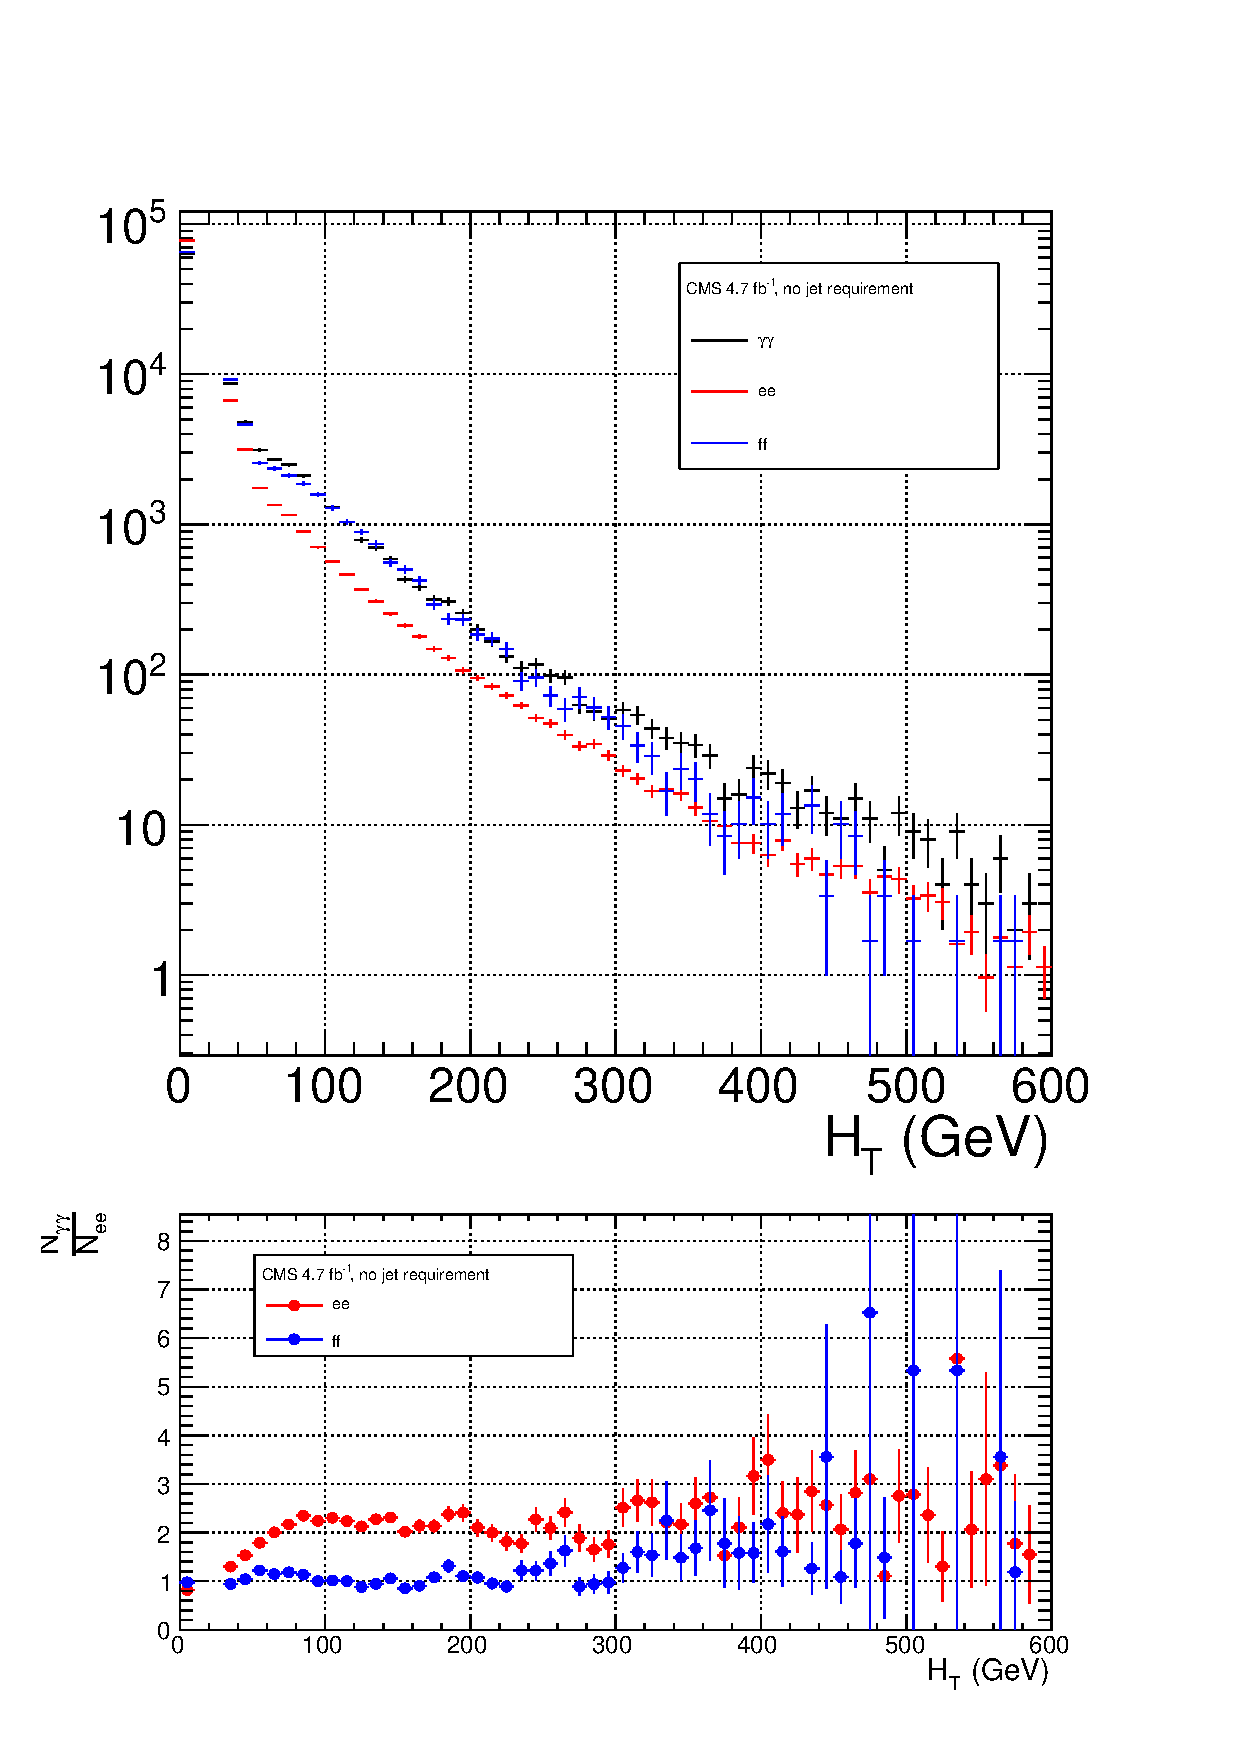
\includegraphics[scale=1.35]{hadronic_activity_HT}}
%	\hspace{1cm}
%	\subfloat[Number of jets per event for jets defined as in Table~\ref{tab:jet_definition}.]{\label{fig:hadronic_activity_Nj}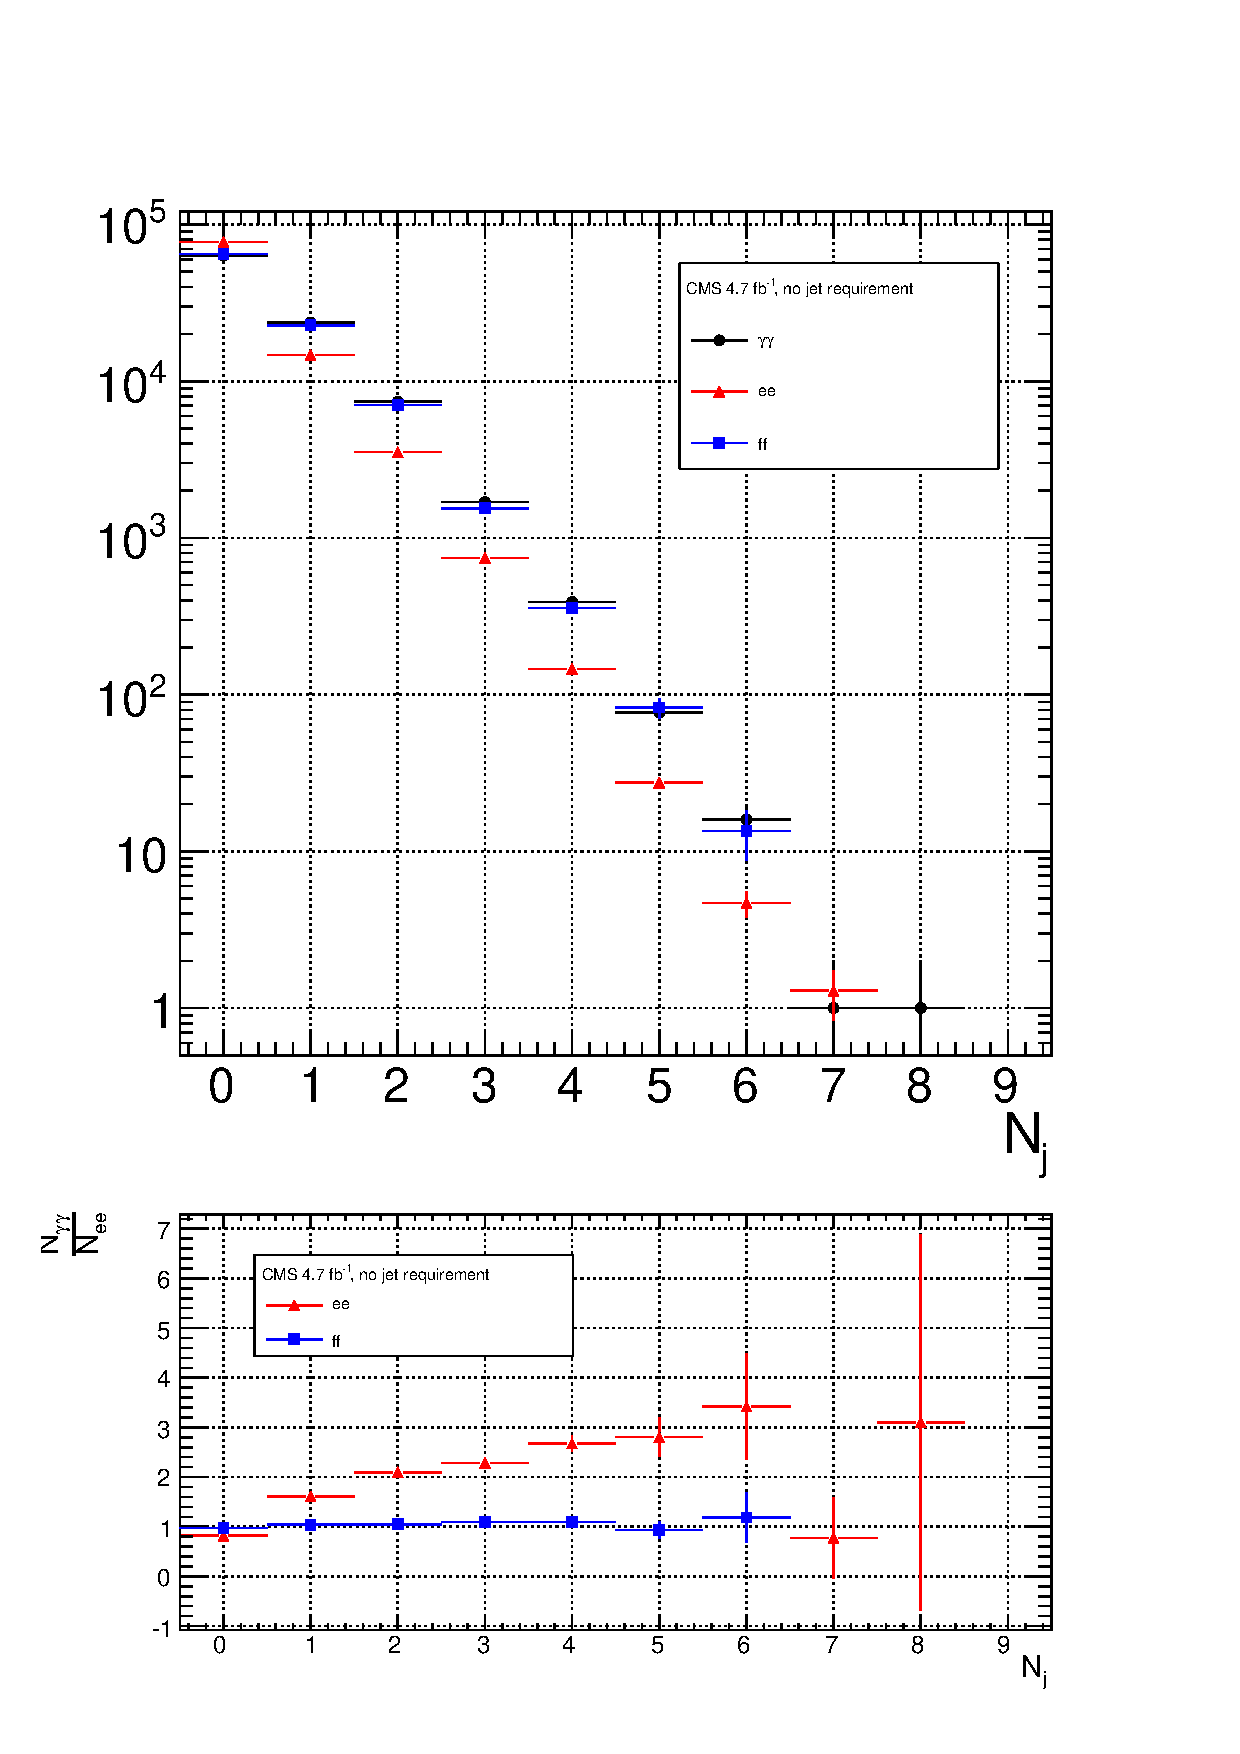
\includegraphics[scale=1.35]{hadronic_activity_Nj}}
%	\\
%	\subfloat[$\not\!\! H_{T}$, defined as the magnitude of the negative vectorial sum of corrected jet $E_{T}$ for jets defined as in Table~\ref{tab:jet_definition}.]{\label{fig:hadronic_activity_MHT}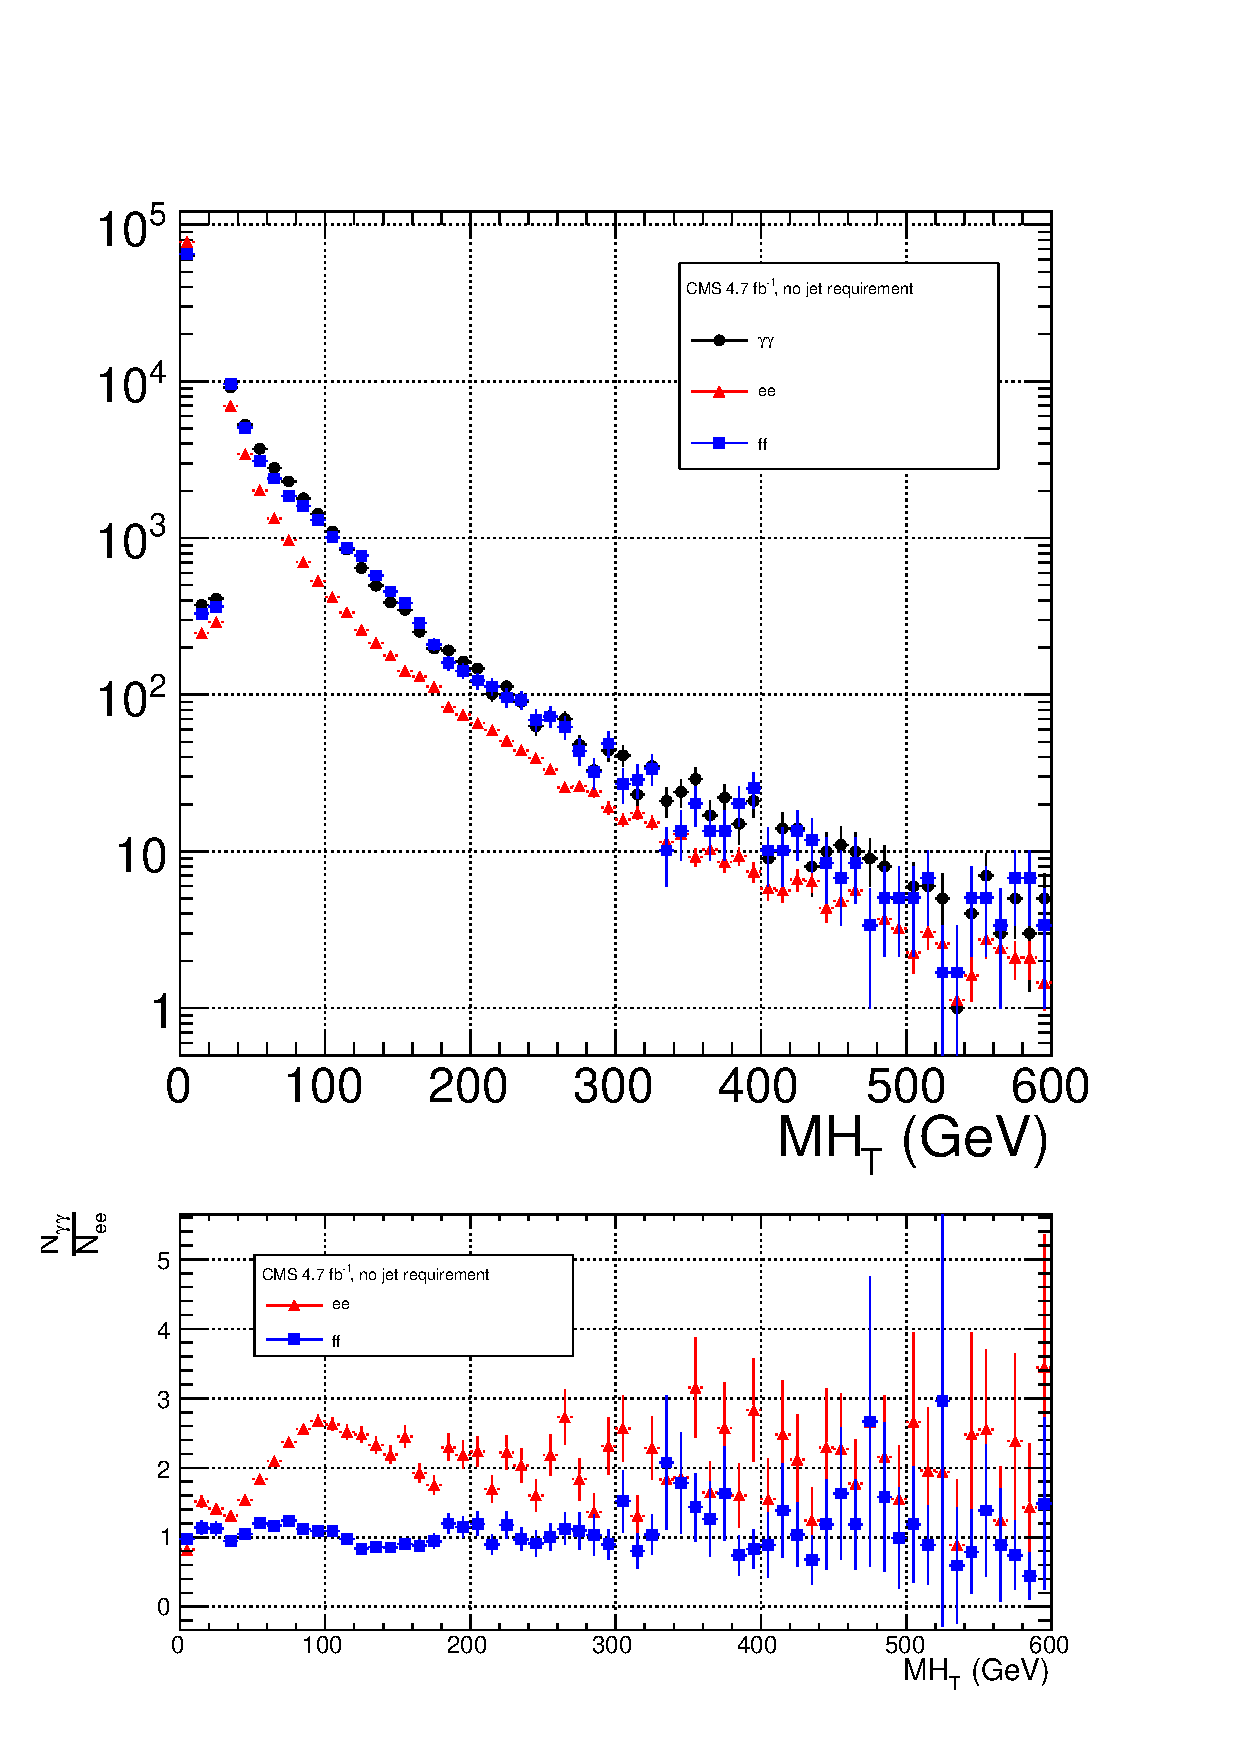
\includegraphics[scale=1.35]{hadronic_activity_MHT}}
%	\hspace{1cm}
%	\subfloat[Corrected $E_{T}$ for the jet with the largest corrected $E_{T}$ per event, for jets defined as in Table~\ref{tab:jet_definition} (excluding the $p_{T}$ requirement).]{\label{fig:hadronic_activity_j1ET}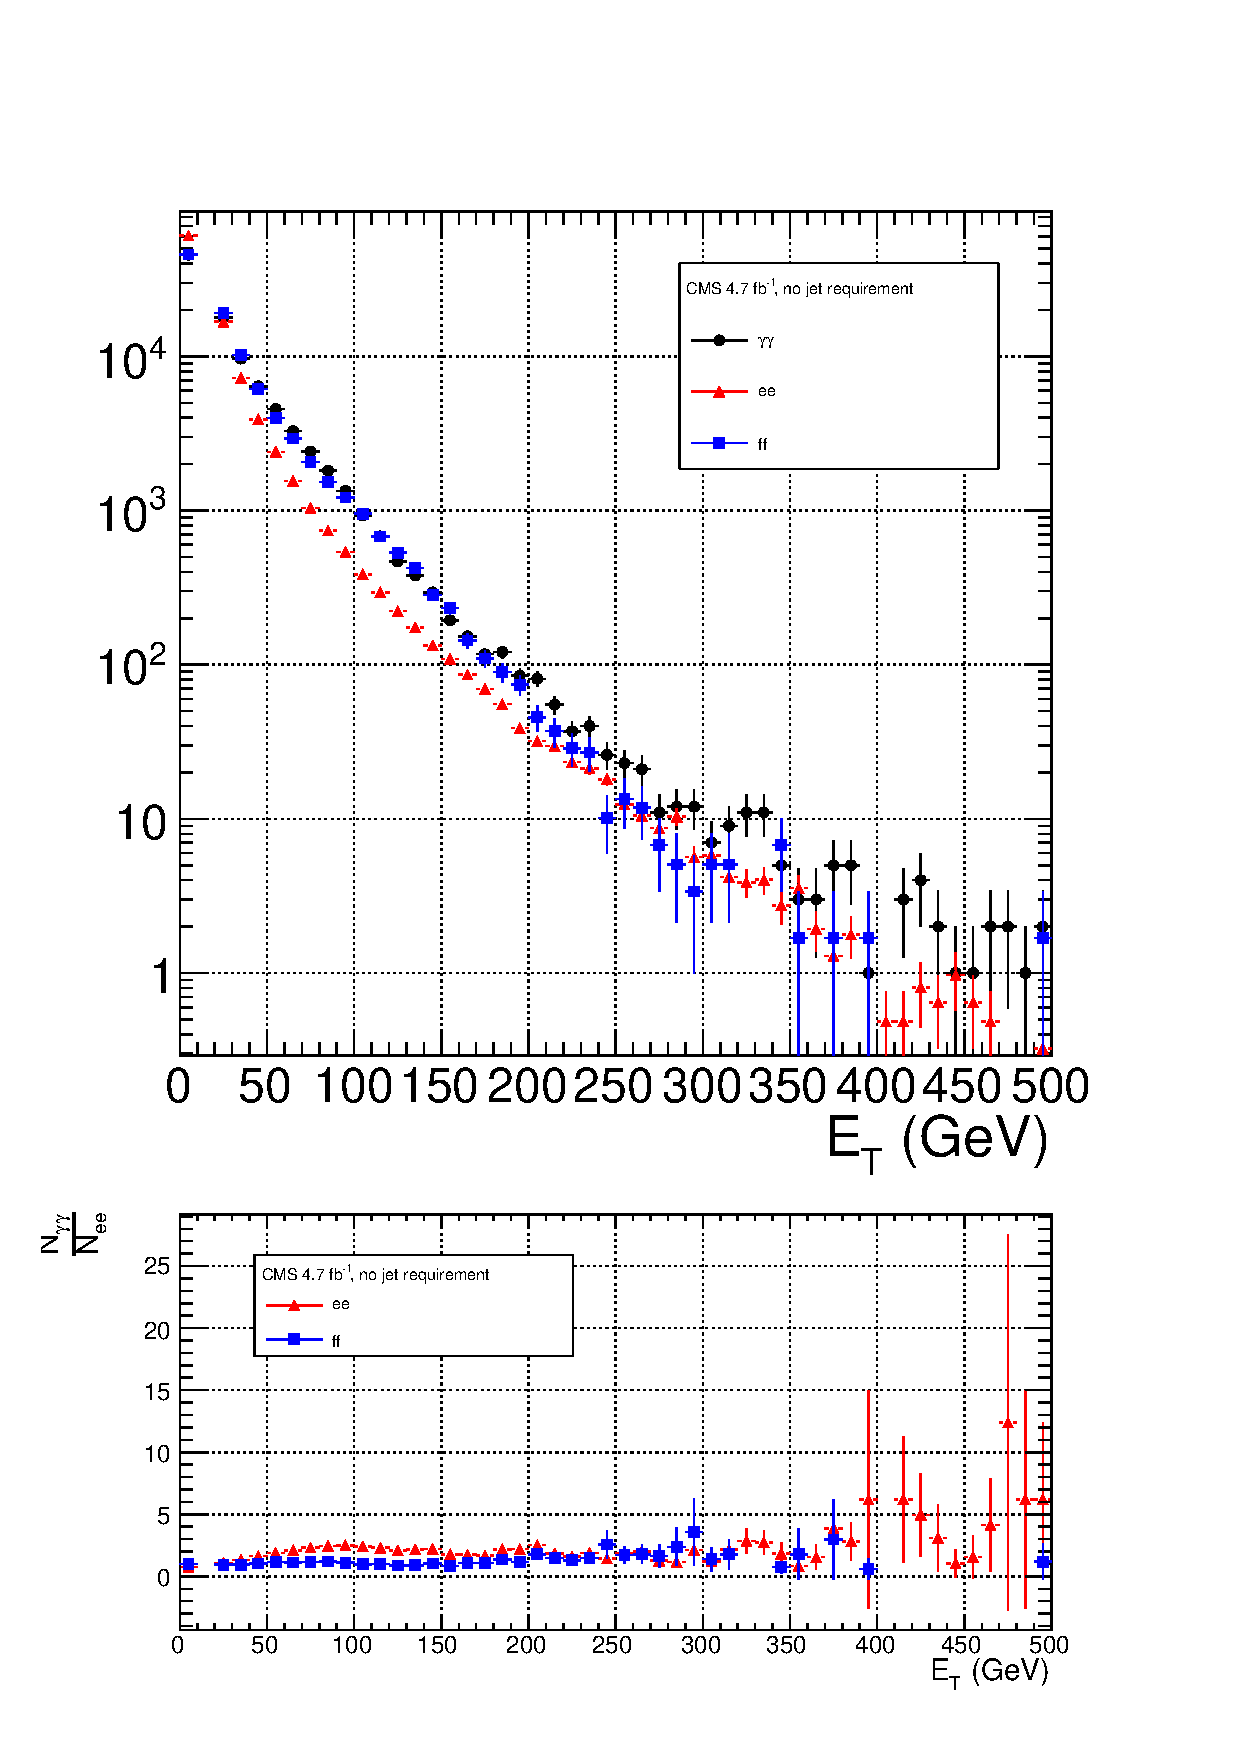
\includegraphics[scale=1.35]{hadronic_activity_j1ET}}
%	\\
%	\subfloat[$\rho$ (average pileup energy density in the calorimeters per unit $\eta\cdot\phi$, cf. Sec.~\ref{sec:Photons}).]{\label{fig:hadronic_activity_rho}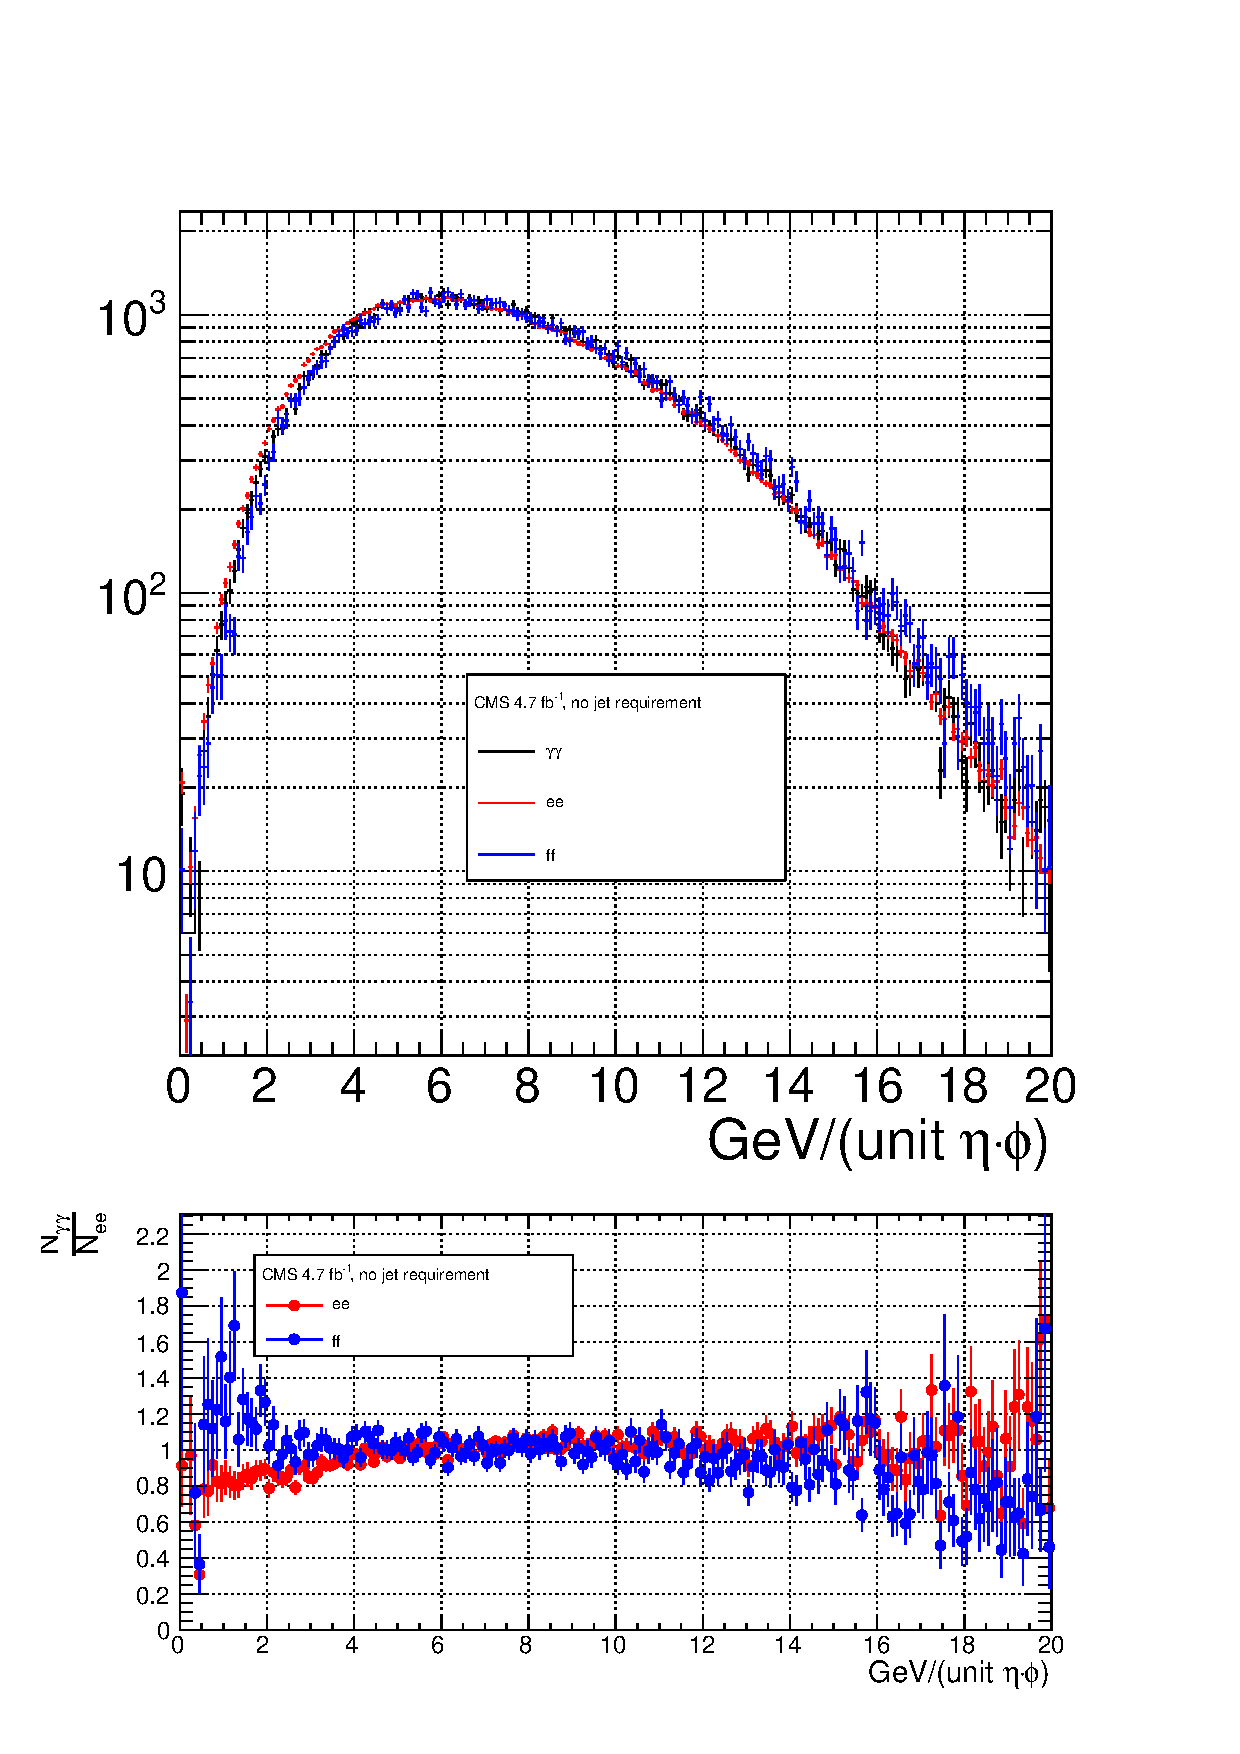
\includegraphics[scale=1.35]{hadronic_activity_rho}}
%	\caption{Comparison of the shapes of some distributions relevant to hadronic activity between the $\gamma\gamma$, $ee$, and $\mathit{ff}$ samples.  The $ee$ and $\mathit{ff}$ distributions are normalized to the number of events in the $\gamma\gamma$ distribution.}
%	\label{fig:hadronic_activity}
%\end{figure}

%add a footnote describing the PF electron and PF muon definitions, with references
\begin{table}[hcbp]
\caption{Definition of hadronic jets.  \textcolor{red}{\textbf{Add a footnote describing the PF electron and PF muon definitions, with references.}}}
\centering
\begin{tabular}{|c|c|}
\hline
Variable & Cut \\
\hline
\hline
Algorithm & \verb+L1FastL2L3Residual+ corrected PF (cf. Sec.~\ref{sec:Jets and Missing Transverse Energy}) \\
\hline
$p_{T}$ & $> 30$ GeV \\
\hline
$|\eta|$ & $< 5.0$ \\
\hline
\begin{tabular}[c]{@{}c@{}}Neutral hadronic\\energy fraction\end{tabular} & $< 0.99$ \\
\hline
\begin{tabular}[c]{@{}c@{}}Neutral electromagnetic\\energy fraction\end{tabular} & $< 0.99$ \\
\hline
Number of constituents & $> 1$ \\
\hline
Charged hadronic energy & $> 0.0$ GeV if $|\eta|  < 2.4$ \\
\hline
Number of charged hadrons & $> 0$ if $|\eta|  < 2.4$ \\
\hline
\begin{tabular}[c]{@{}c@{}}Charged electromagnetic\\energy fraction\end{tabular} & $< 0.99$ if $|\eta| < 2.4$ \\
\hline
\begin{tabular}[c]{@{}c@{}}$\Delta R$ to nearest electron, muon,\\or one of the two\\primary EM objects\end{tabular} & $> 0.5$ \\
\hline
\end{tabular}
\label{tab:jet_definition}
\end{table}

\subsection{Reweighting}
\label{sec:Reweighting}

To reweight the control sample events to match the kinematics of the candidate sample events, a weight based on the $p_{T}$ of the di-EM-object system and the number of jets in the event is used.  As explained in Sec.~\ref{sec:Outline of the Procedure}, \MET in the $\gamma\gamma$, $\mathit{ff}$, and $ee$ samples is due to the poorly measured hadronic recoil off the well-measured di-EM system.  Therefore, the $p_{T}$ of the di-EM system is a good handle on the true magnitude of the hadronic recoil, which affects the measured \MET.  The di-EM system is depicted in Figure~\ref{fig:di-EM_pT_cartoon}.

\begin{figure}
	\centering
	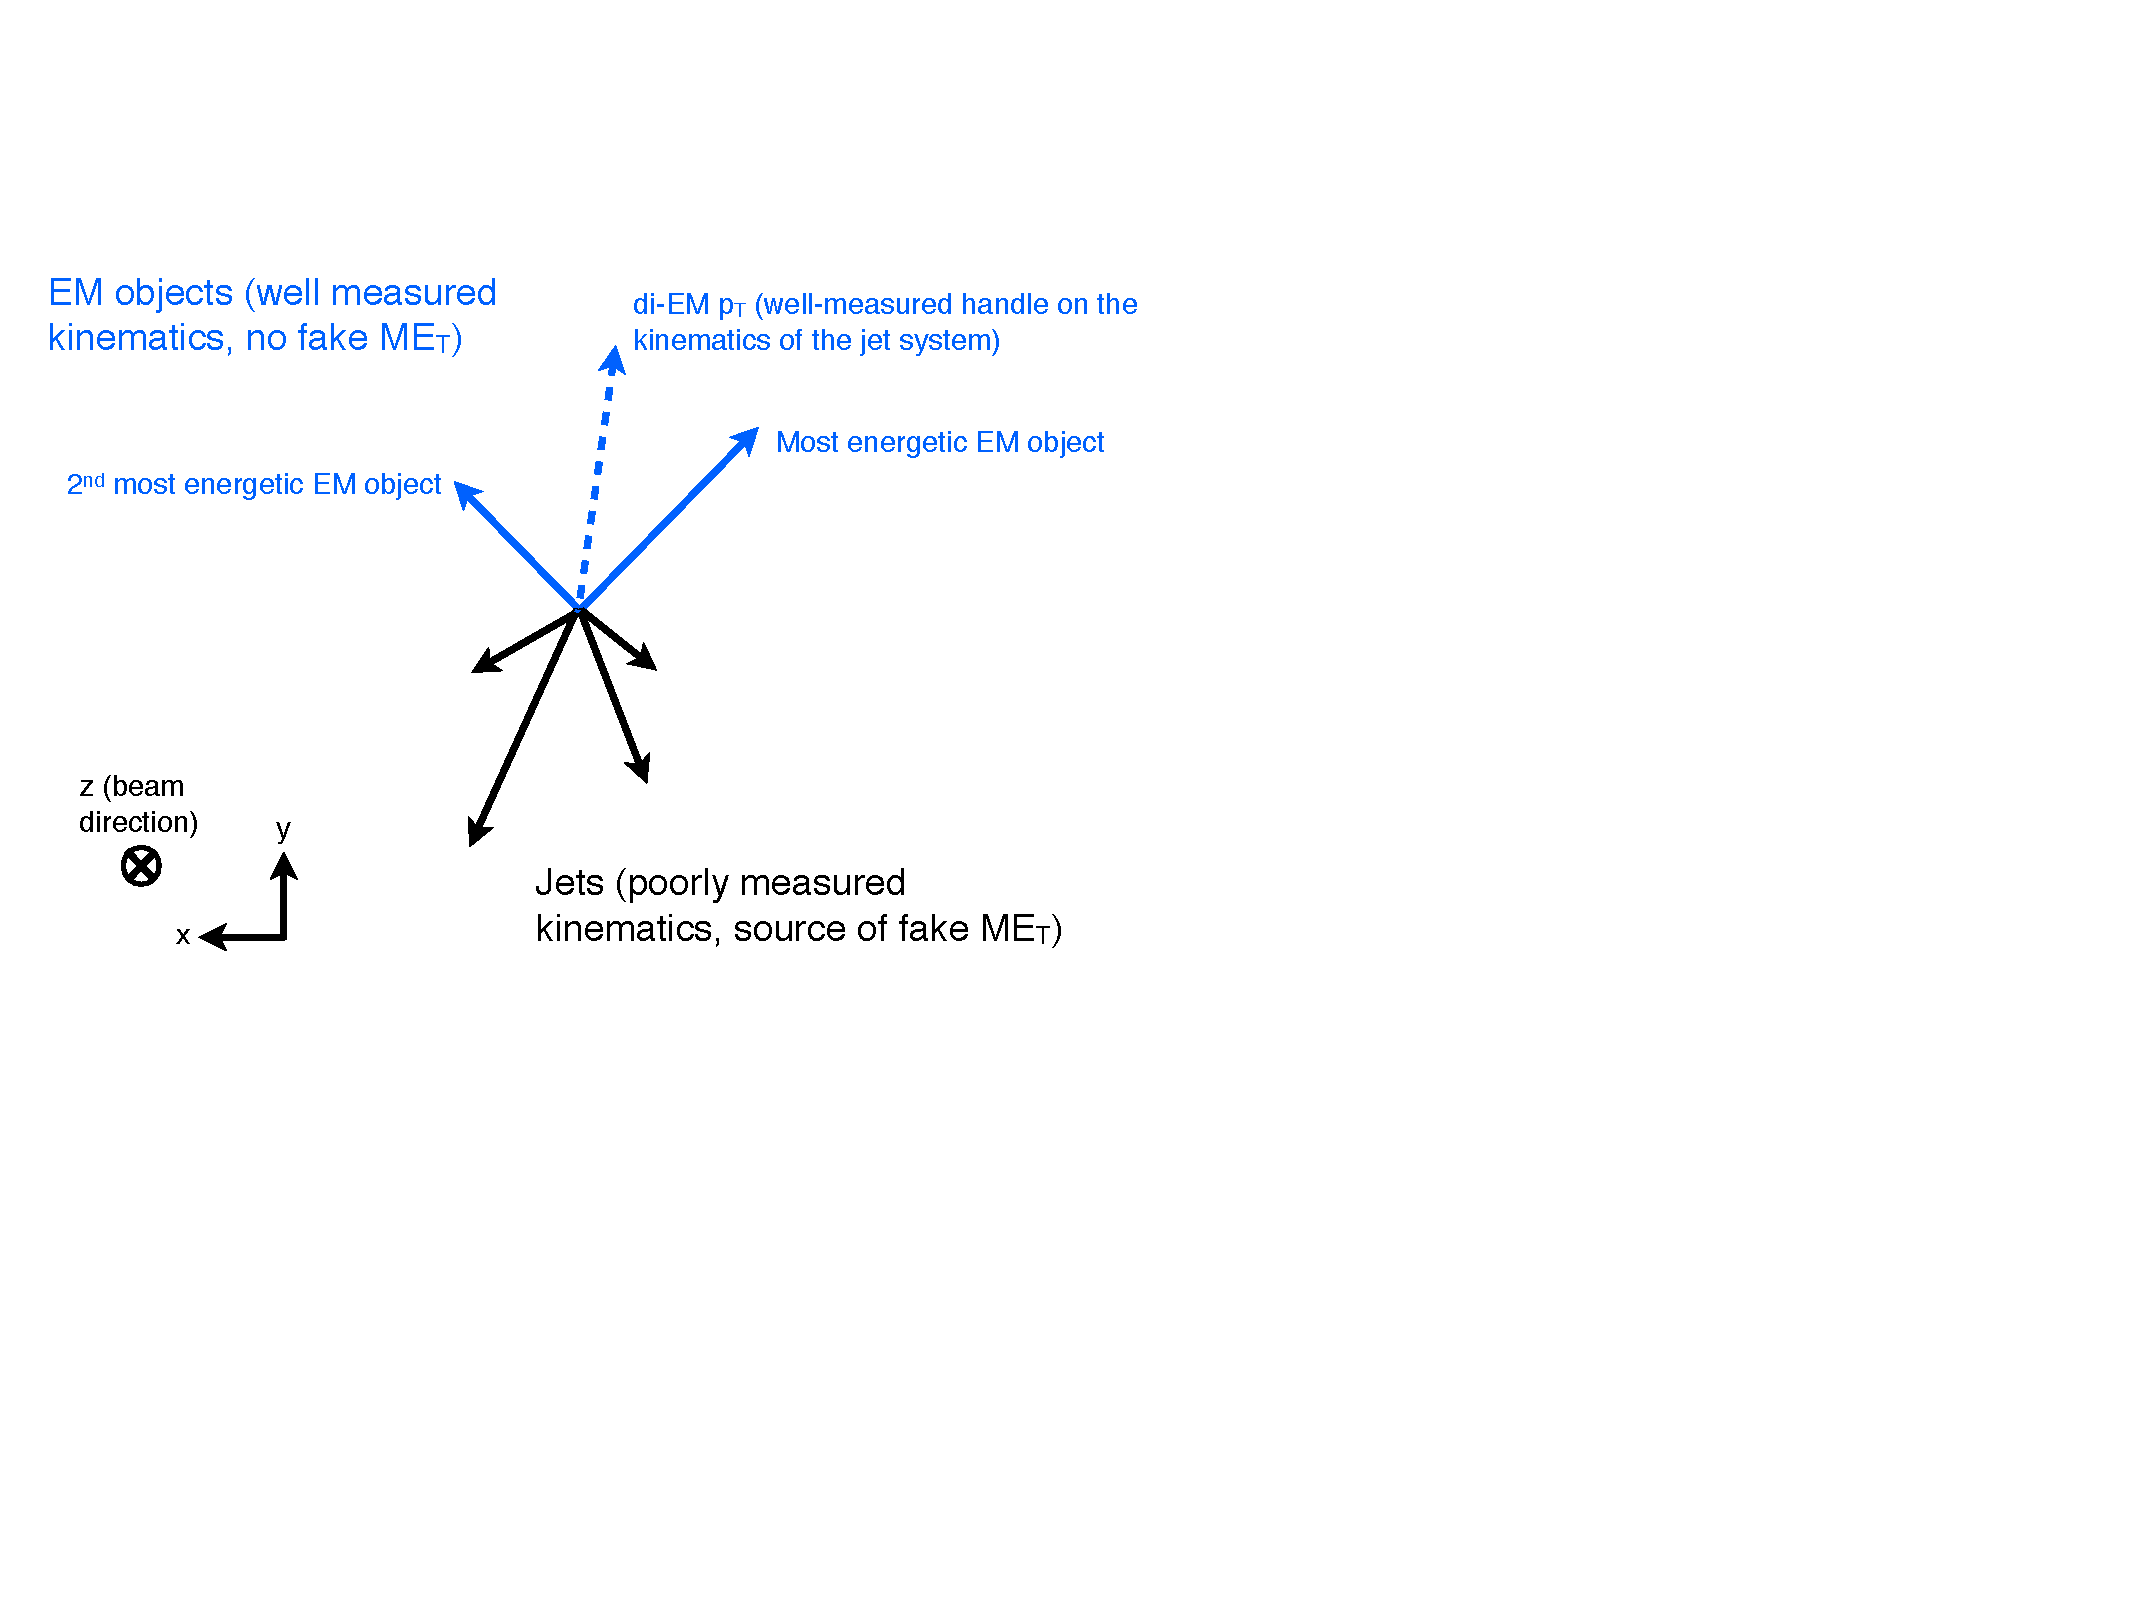
\includegraphics[scale=0.5]{di-EM_pT_cartoon}
	\caption{Cartoon showing the di-EM system in blue and the hadronic recoil in black.  The di-EM $p_{T}$ (dashed blue line) is used to reweight the control sample kinematic properties to match those of the candidate $\gamma\gamma$ sample.}.
	\label{fig:di-EM_pT_cartoon}
\end{figure}

Whereas the di-EM $p_{T}$ reweighting accounts for differences in production kinematics between the control and $\gamma\gamma$ samples, a simultaneous reweighting based on the number of jets in the event accounts for differences in hadronic activity between the samples, especially between $ee$ and $\gamma\gamma$ (cf. Fig.~\ref{fig:hadronic_activity}).  Jets are defined as in Table~\ref{tab:jet_definition}, but with $|\eta|$ restricted to 2.6 (i.e. HF jets excluded).  Figure~\ref{fig:dijet_pT_and_Nj_vs_dijet_pT_reweighting} shows the effect of reweighting by number of jets per event, which is to increase(decrease) the tail of the $ee$($\mathit{ff}$) \MET spectrum.

%include ee/gg and ff/gg agreement?
%\begin{figure}
%	\centering
%	\subfloat[$ee$ \MET spectra.]{\label{fig:ee_dijet_pT_and_Nj_vs_dijet_pT_reweighting}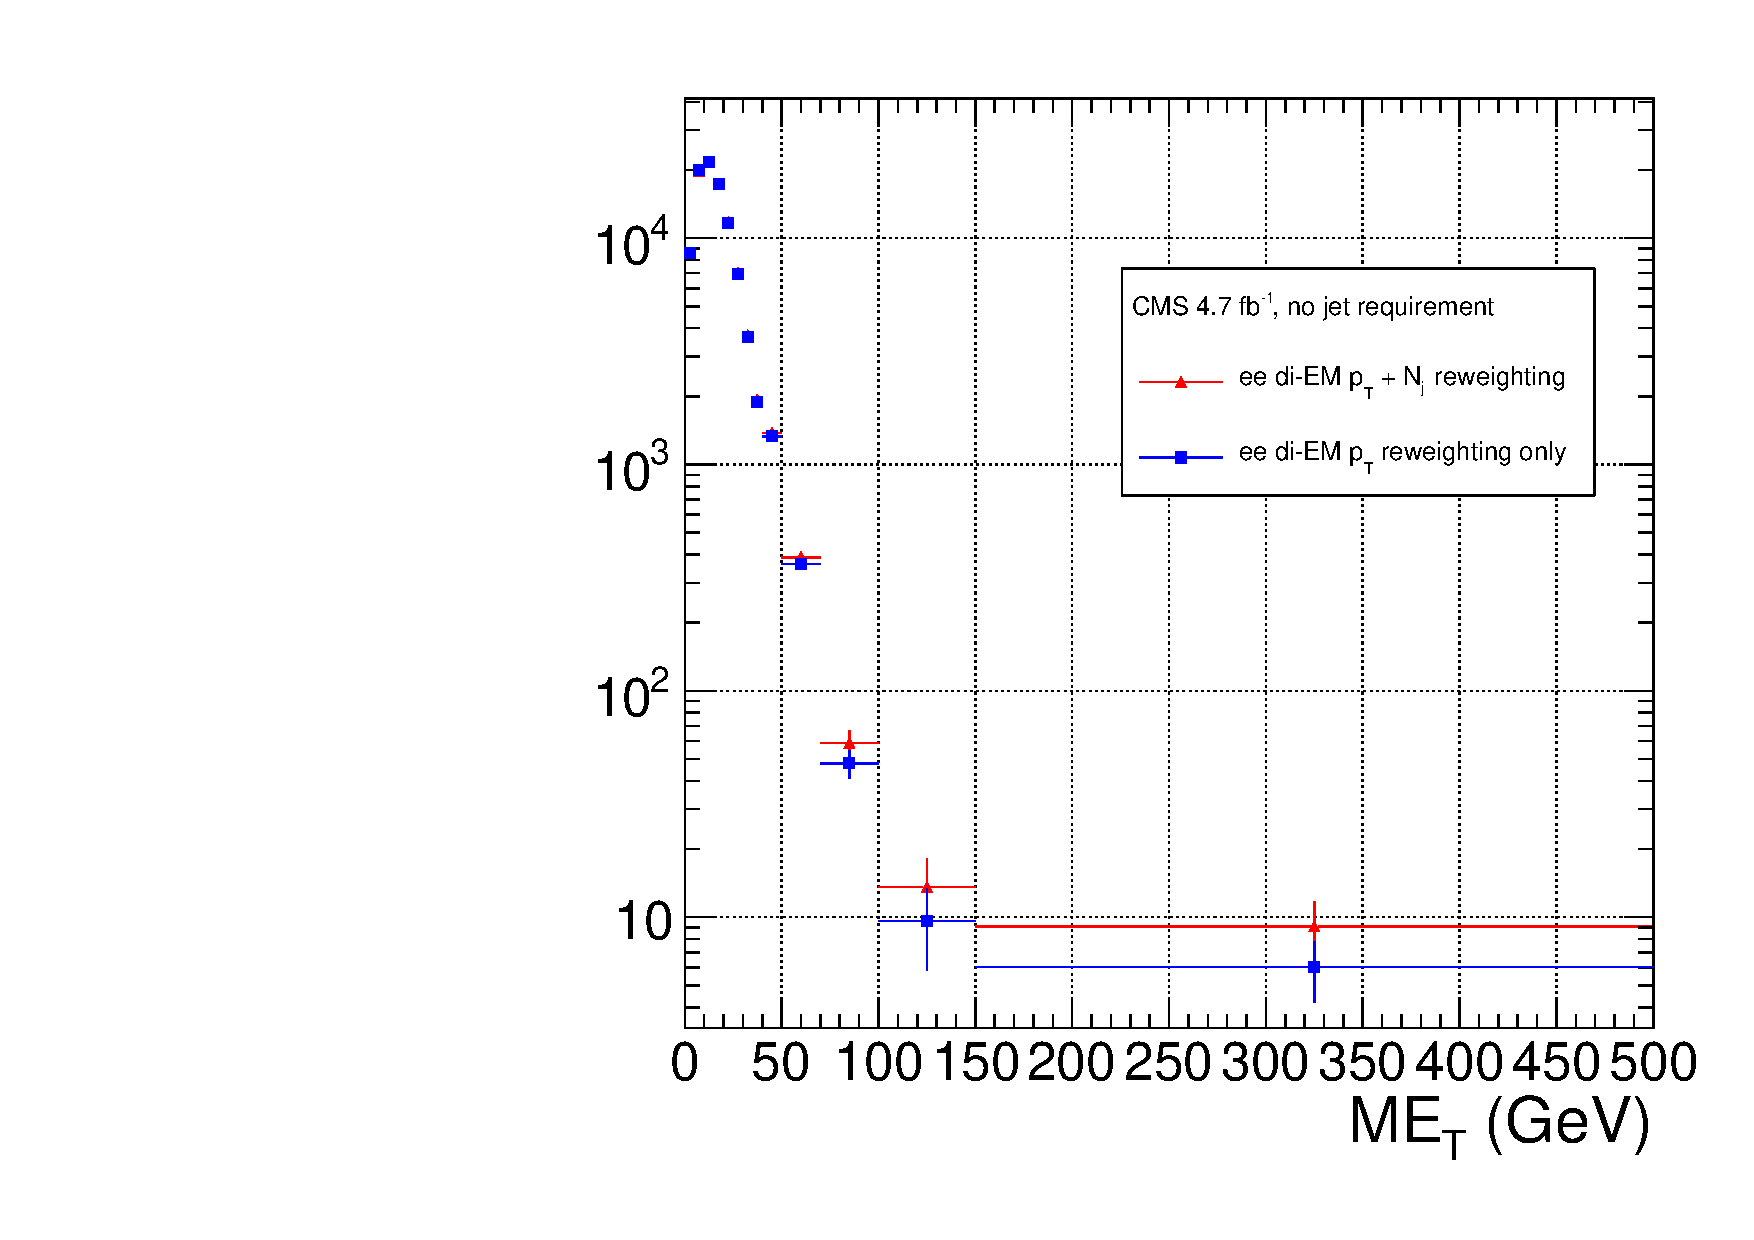
\includegraphics[scale=0.25]{ee_dijet_pT_and_Nj_vs_dijet_pT_reweighting}}
%	\hspace{1cm}
%	\subfloat[$\mathit{ff}$ \MET spectra.]{\label{fig:ff_dijet_pT_and_Nj_vs_dijet_pT_reweighting}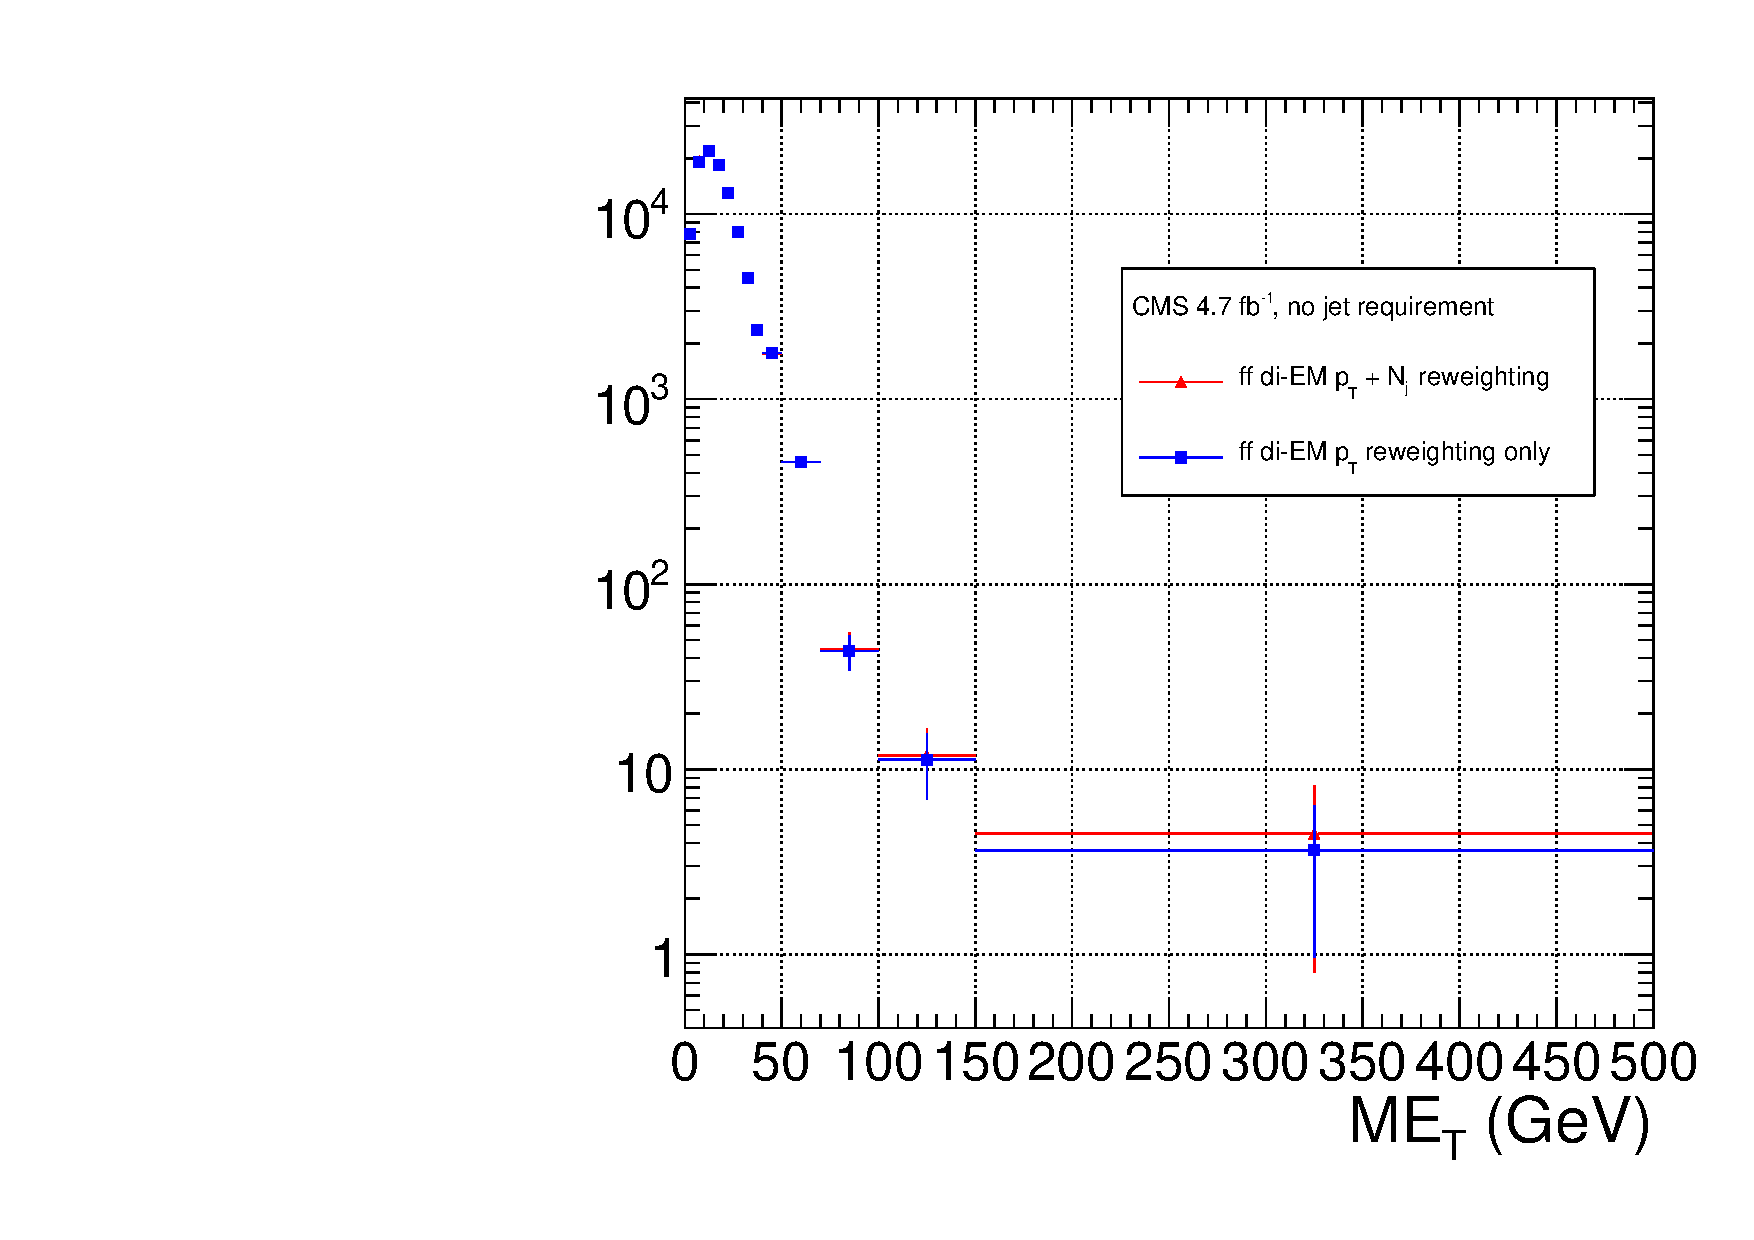
\includegraphics[scale=0.25]{ff_dijet_pT_and_Nj_vs_dijet_pT_reweighting}}
%	\\
%	\subfloat[Ratio of $ee$ to $\mathit{ff}$ \MET spectra for di-EM $p_{T}$ reweighting only (red) and di-EM $p_{T}$ + number of jets reweighting (blue).]{\label{fig:ee_over_ff_dijet_pT_and_Nj_vs_dijet_pT_reweighting}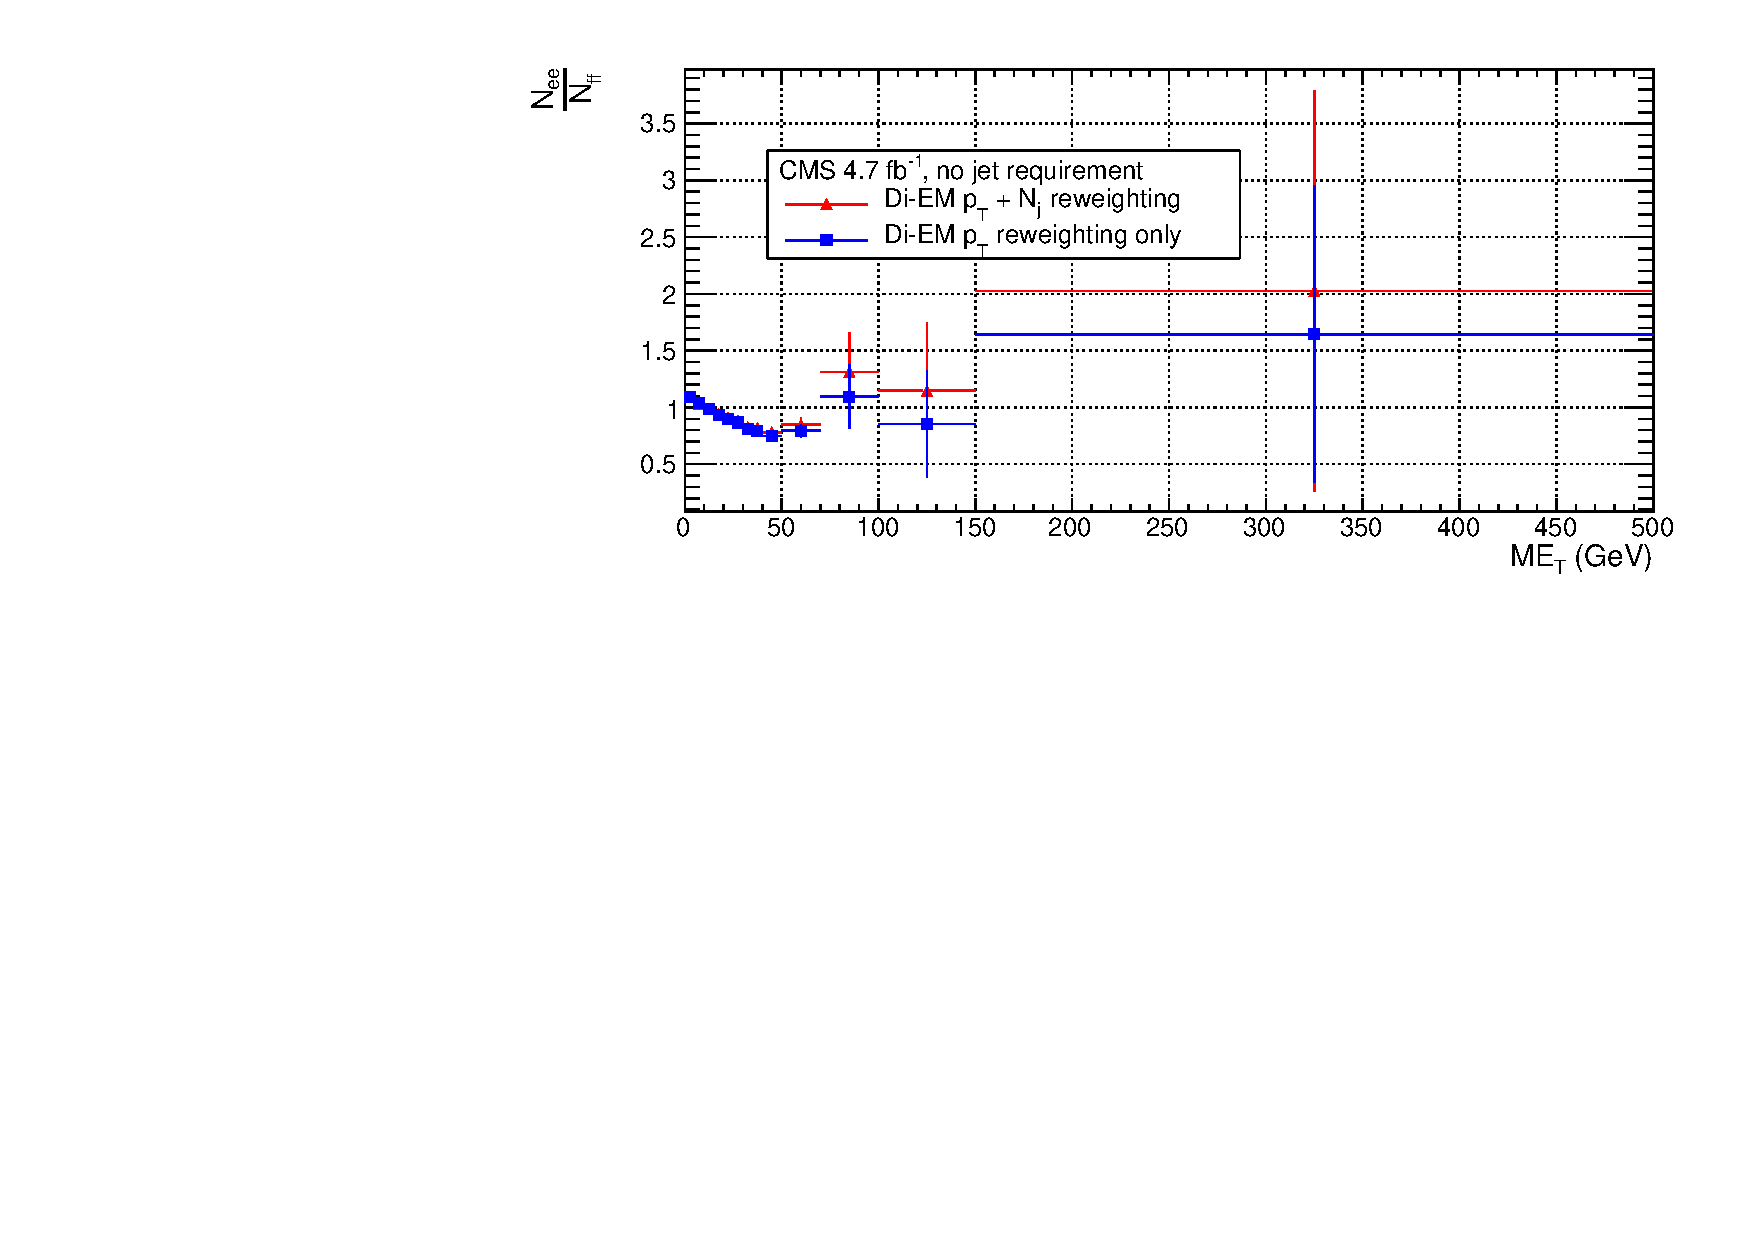
\includegraphics[scale=0.25]{ee_over_ff_dijet_pT_and_Nj_vs_dijet_pT_reweighting}}
%	\caption{\MET spectra of the reweighted $ee$ and $\mathit{ff}$ control samples.  Squares indicate di-EM $p_{T}$ reweighting only; triangles indicate di-EM $p_{T}$ + number of jets reweighting.  PF $p_{T}$ (cf. p.~\pageref{fig:ET_bias_vs_EMF}) is used to calculate the di-EM $p_{T}$.  The full normalization procedure is employed, along with $ee$ sideband subtraction (discussed in Sec.~\ref{sec:ee Control Sample}).}
%	\label{fig:dijet_pT_and_Nj_vs_dijet_pT_reweighting}
%\end{figure}

Although the electron and photon energies are well measured by the ECAL, the ECAL-only measurement of the fake photon energy (cf. Sec~\ref{sec:Photons}) is biased slightly low due to the fact that fakes (which are really jets) tend to deposit some energy in the HCAL.  This can be seen in Figs.~\ref{fig:ET_bias_vs_EMF} and~\ref{fig:4684pb-1_single_ETBias}, which show the relative difference between the ECAL-only $E_{T}$ measurement and the PF $E_{T}$ measurement vs. EMF for electrons, photons, and fakes.  PF $E_{T}$ is defined as the \verb+L1Fast+-corrected $E_{T}$ of the nearest PF jet with $p_{T} \geq 20$ GeV (i.e., the $E_{T}$ of the PF jet object reconstructed from the same ECAL shower as the fake photon).  On average, the fakes tend to deposit a few percent more energy in the HCAL than the electrons or photons, which is recovered by the PF algorithm.  For this reason, the PF $p_{T}$ is used in the calculation of di-EM $p_{T}$ rather than the ECAL-only $p_{T}$.  This leads to a modest improvement in the agreement between the $ee$ and $\mathit{ff}$ \MET spectra, as shown in Figure~\ref{fig:ee_vs_ff_di-EM_vs_dijet_pT_reweighting}.

\begin{figure}
	\centering
	\subfloat[Leading electron in $ee$ events.]{\label{fig:4684pb-1_leadingE_ETBias_log}\includegraphics[scale=0.25]{4684pb-1_leadingE_ETBias_log}}
	\hspace{1cm}
	\subfloat[Trailing electron in $ee$ events.]{\label{fig:4684pb-1_trailingE_ETBias_log}\includegraphics[scale=0.25]{4684pb-1_trailingE_ETBias_log}}
	\\
	\subfloat[Leading fake in $\mathit{ff}$ events.]{\label{fig:4684pb-1_leadingF_ETBias_log}\includegraphics[scale=0.25]{4684pb-1_leadingF_ETBias_log}}
	\hspace{1cm}
	\subfloat[Trailing fake in $\mathit{ff}$ events.]{\label{fig:4684pb-1_trailingF_ETBias_log}\includegraphics[scale=0.25]{4684pb-1_trailingF_ETBias_log}}
	\\
	\subfloat[Leading photon in $\gamma\gamma$ events.]{\label{fig:4684pb-1_leadingG_ETBias_log}\includegraphics[scale=0.25]{4684pb-1_leadingG_ETBias_log}}
	\hspace{1cm}
	\subfloat[Trailing photon in $\gamma\gamma$ events.]{\label{fig:4684pb-1_trailingG_ETBias_log}\includegraphics[scale=0.25]{4684pb-1_trailingG_ETBias_log}}
	\caption{Relative difference between the ECAL-only $E_{T}$ measurement and the PF $E_{T}$ measurement vs. EMF.  PF $E_{T}$ is defined in the text.  \textcolor{red}{\textbf{Replace with current figure.}}}
	\label{fig:ET_bias_vs_EMF}
\end{figure}

\begin{figure}
	\centering
	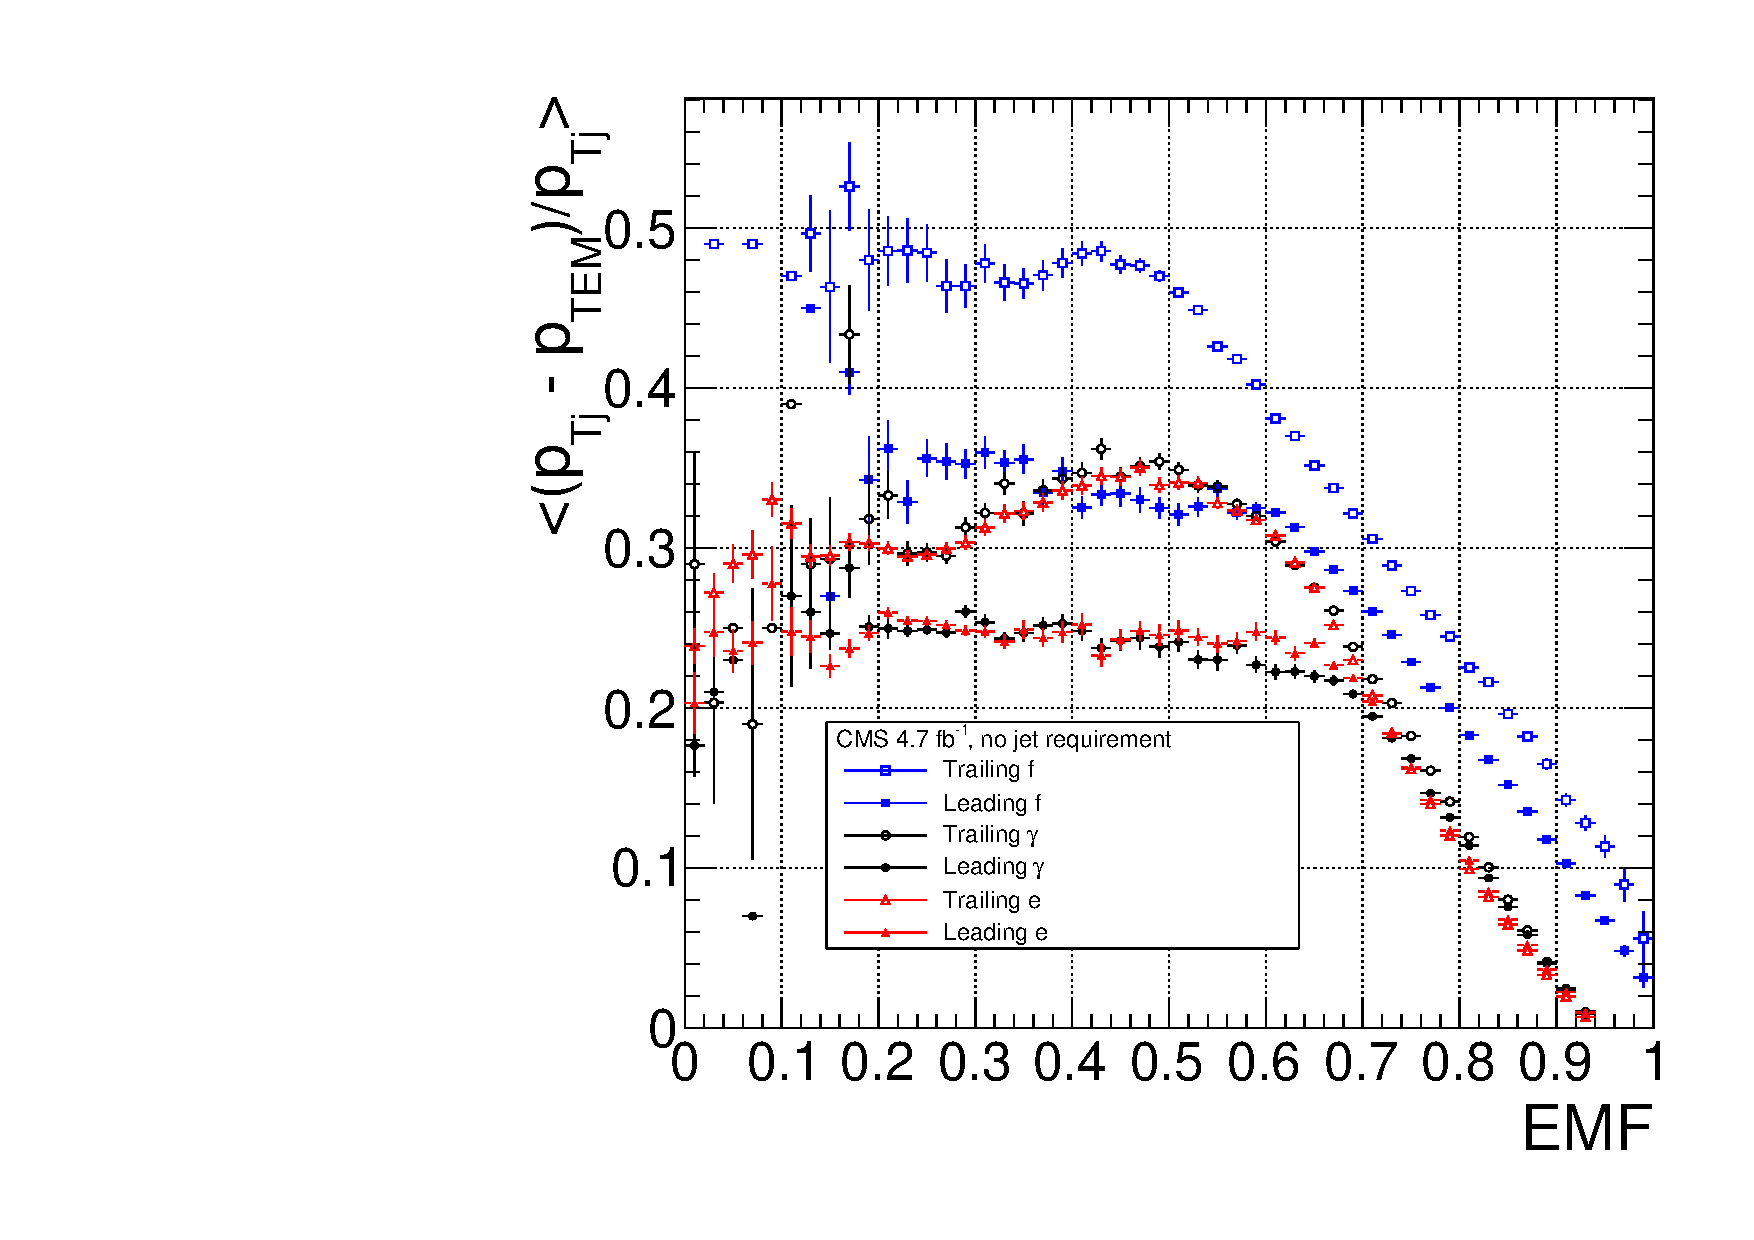
\includegraphics[scale=0.5]{4684pb-1_single_ETBias}
	\caption{Average relative difference between the ECAL-only $E_{T}$ measurement and the PF $E_{T}$ measurement vs. EMF for the two electrons in $ee$ events, the two fakes in $\mathit{ff}$ events, and the two photons in $\gamma\gamma$ events (i.e. profile histograms of Fig.~\ref{fig:ET_bias_vs_EMF}).  PF $E_{T}$ is defined in the text.  \textcolor{red}{\textbf{Replace with current figure.}}}
	\label{fig:4684pb-1_single_ETBias}
\end{figure}

%include ee/gg and ff/gg agreement?
%\begin{figure}
%	\centering
%	\subfloat[$ee$ \MET spectra.]{\label{fig:ee_di-EM_vs_dijet_pT_reweighting}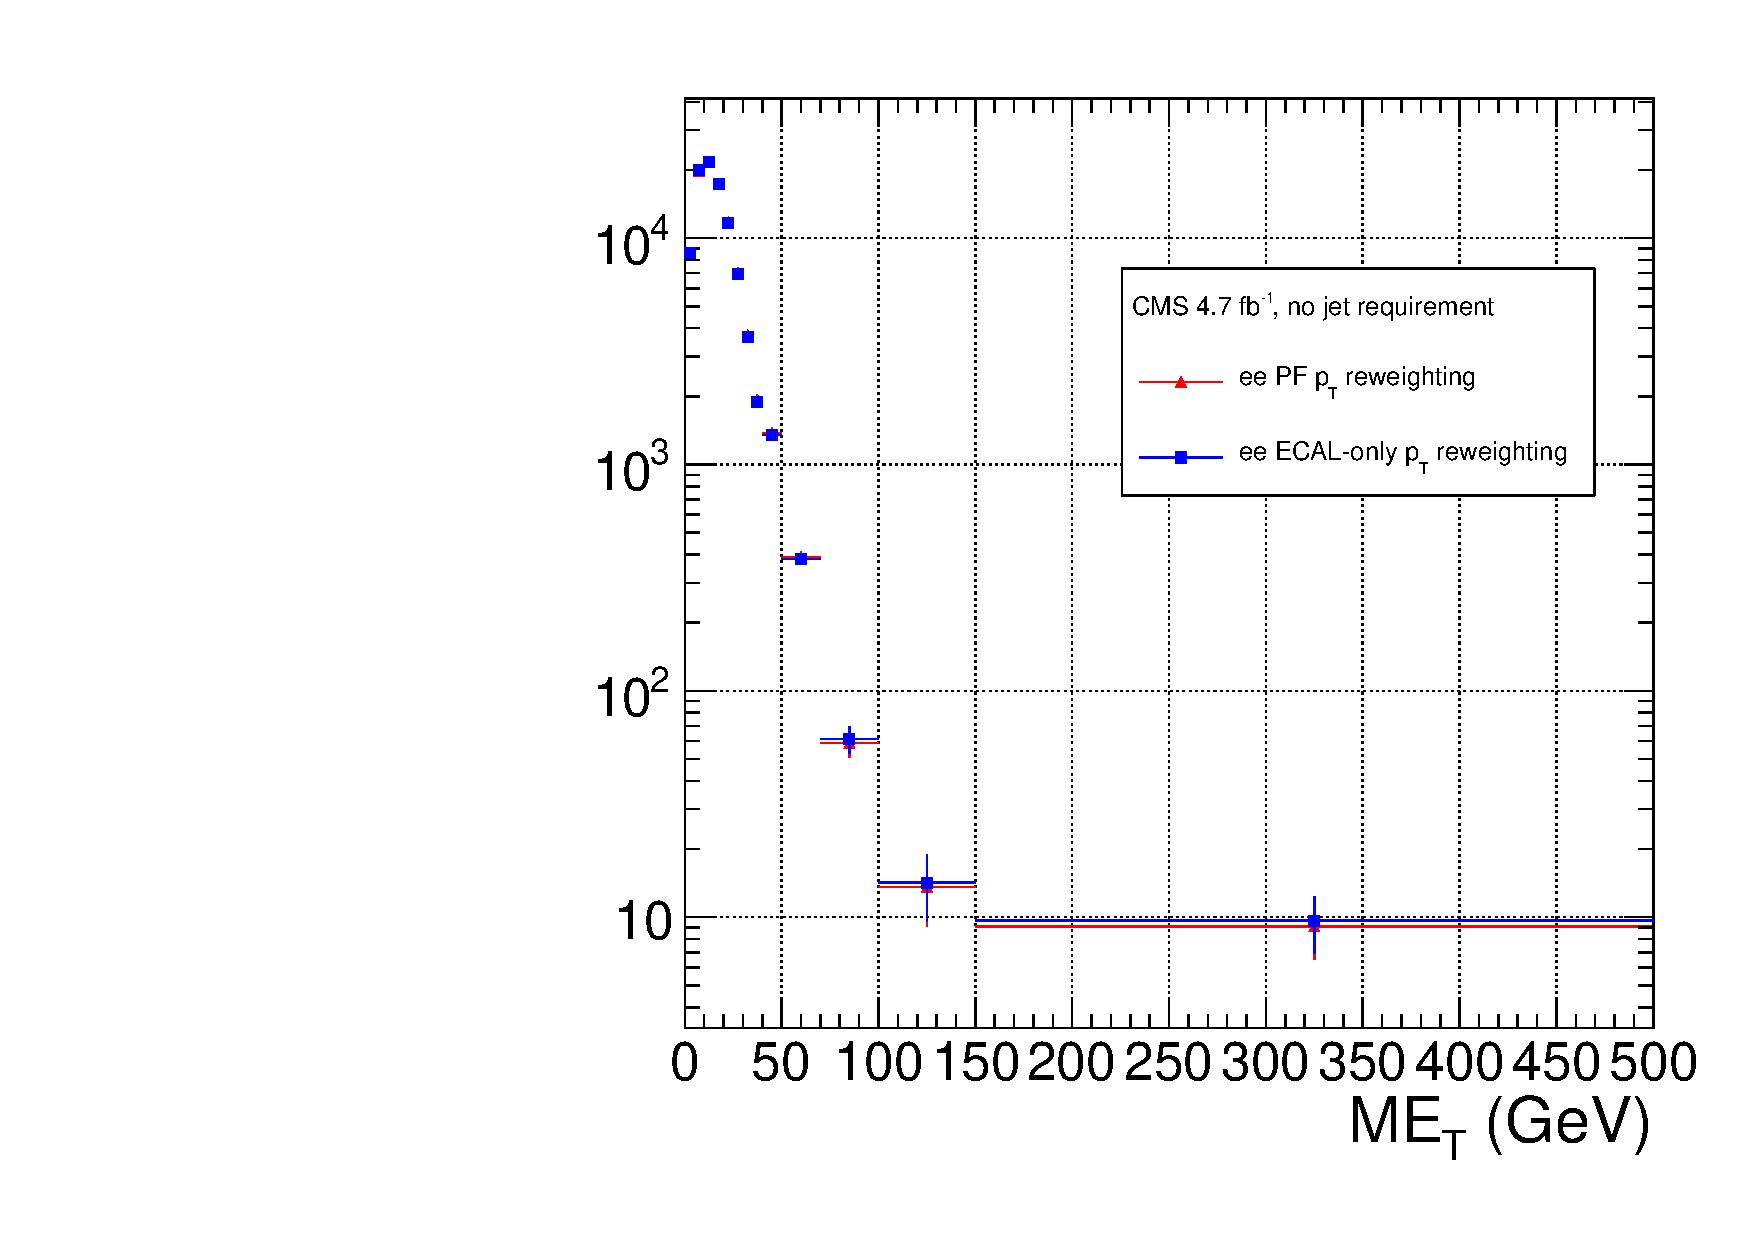
\includegraphics[scale=0.25]{ee_di-EM_vs_dijet_pT_reweighting}}
%	\hspace{1cm}
%	\subfloat[$\mathit{ff}$ \MET spectra.]{\label{fig:ff_di-EM_vs_dijet_pT_reweighting}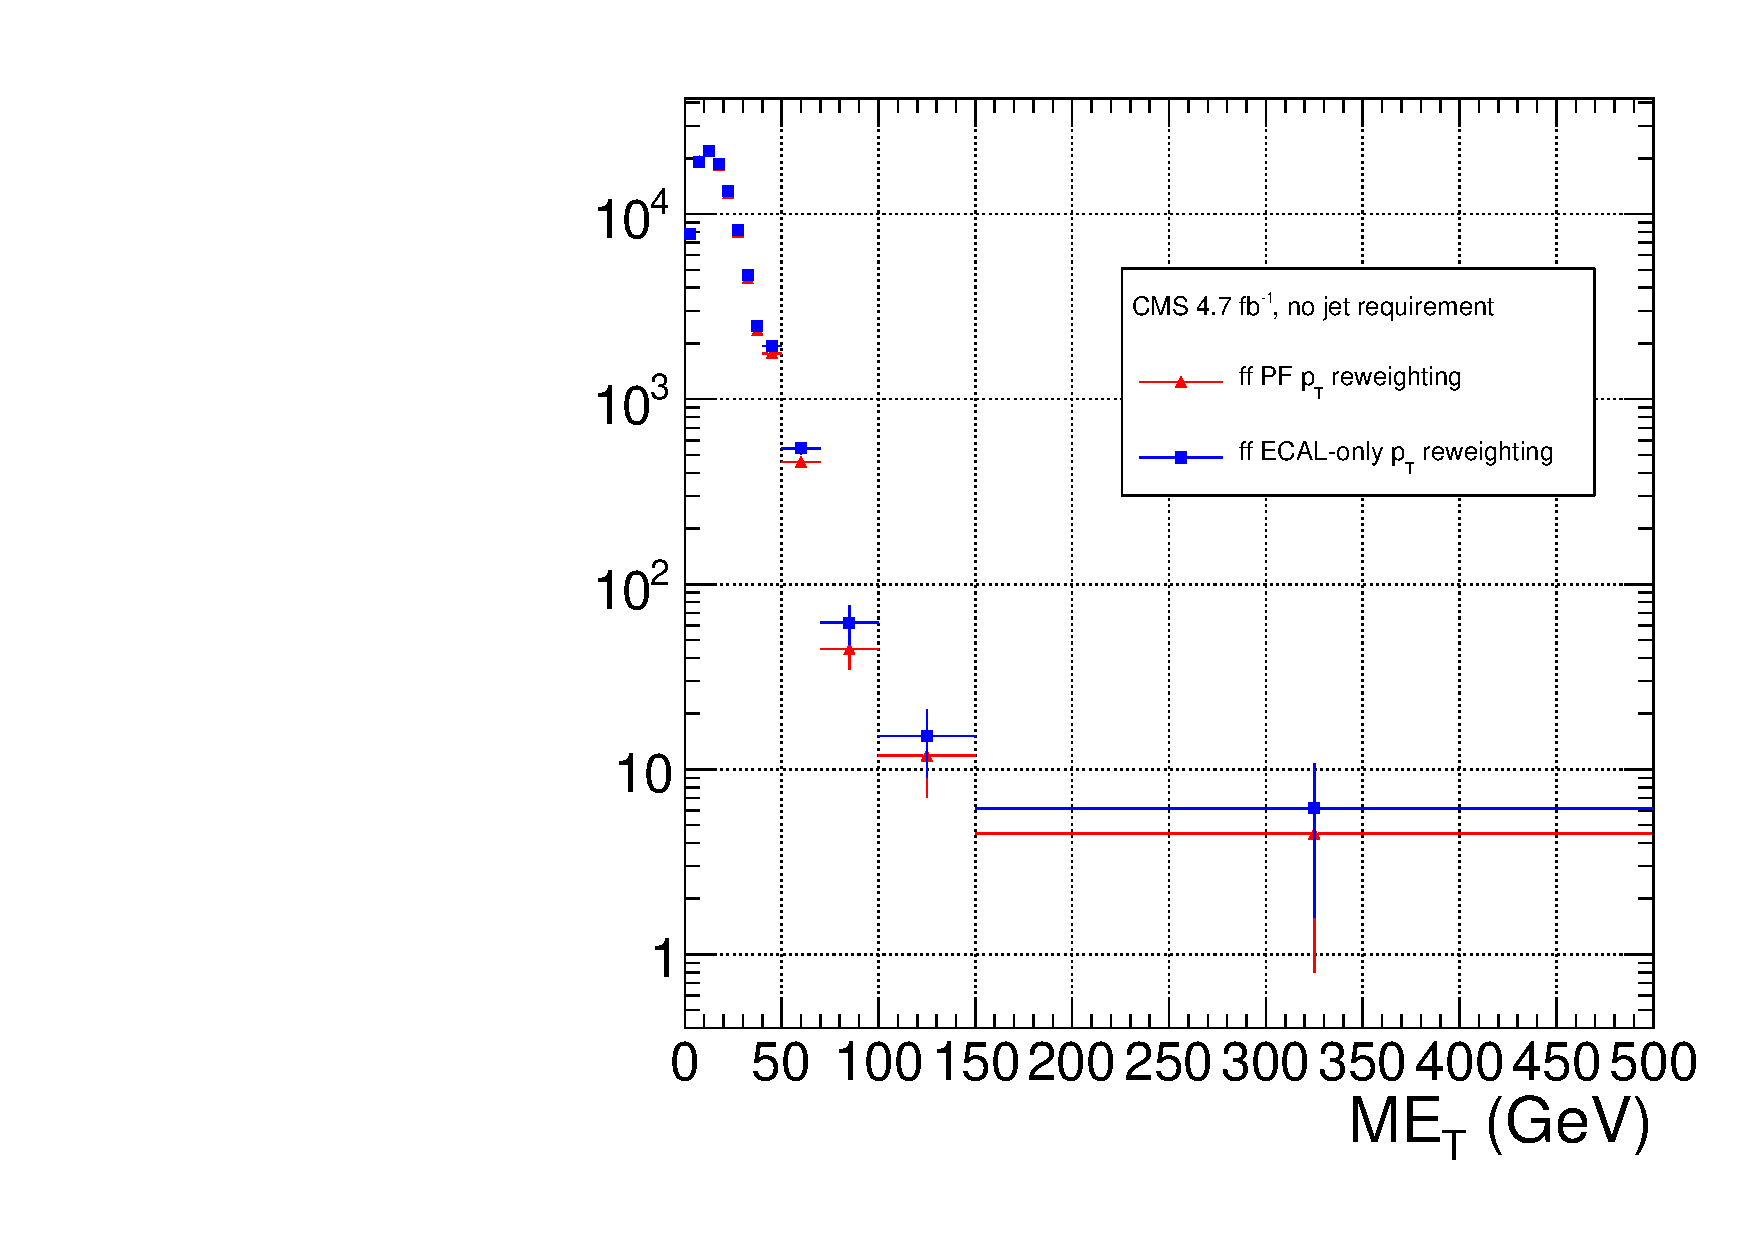
\includegraphics[scale=0.25]{ff_di-EM_vs_dijet_pT_reweighting}}
%	\\
%	\subfloat[Ratio of $ee$ to $\mathit{ff}$ \MET spectra for ECAL-only $p_{T}$ estimate (red) and PF $p_{T}$ estimate (blue).]{\label{fig:ee_over_ff_di-EM_vs_dijet_pT_reweighting}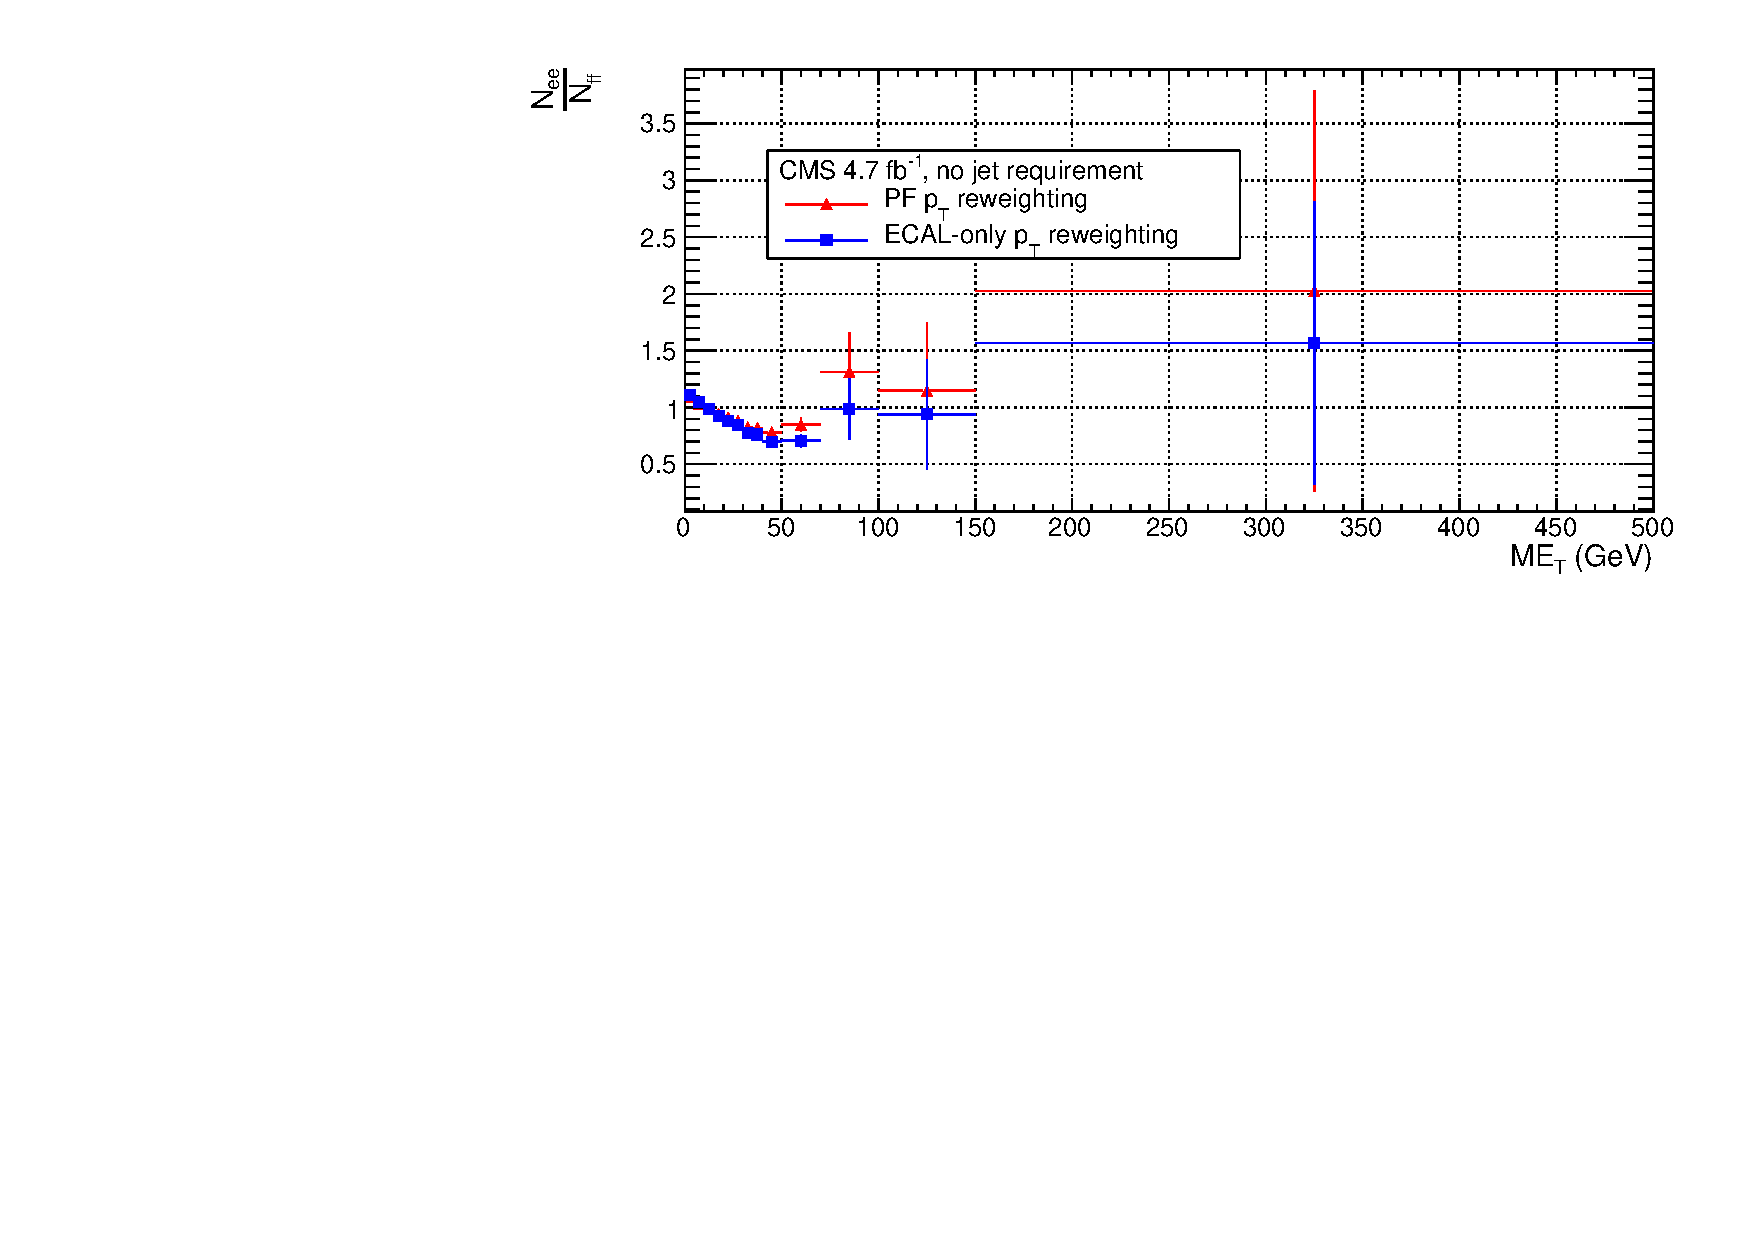
\includegraphics[scale=0.25]{ee_over_ff_di-EM_vs_dijet_pT_reweighting}}
%	\caption{\MET spectra of the reweighted $ee$ and $\mathit{ff}$ control samples.  Squares indicate reweighting using the ECAL-only $p_{T}$ estimate; triangles indicate reweighting using the PF $p_{T}$ estimate.  The full reweighting and normalization procedure is employed, along with $ee$ sideband subtraction (discussed in Sec.~\ref{sec:ee Control Sample}).}
%	\label{fig:ee_vs_ff_di-EM_vs_dijet_pT_reweighting}
%\end{figure}

The control sample event weights are defined as

\begin{eqnarray}
w_{ij} &=& \frac{N_{\mathrm{control}}}{N_{\gamma\gamma}}\frac{N_{\gamma\gamma}^{ij}}{N_{\mathrm{control}}^{ij}}
\end{eqnarray}
%
where $i$ runs over the number of di-EM $p_{T}$ bins, $j$ runs over the number of jet bins, $N_{\mathrm{control}}$ is the total number of events in the control sample, $N_{\gamma\gamma}$ is the total number of events in the $\gamma\gamma$ sample, $N_{\gamma\gamma}^{ij}$ is the number of $\gamma\gamma$ events in the $i^{\mathrm{th}}$ di-EM $p_{T}$ bin and $j^{\mathrm{th}}$ jet bin, and $N_{\mathrm{control}}^{ij}$ is the number of control sample events in the $i^{\mathrm{th}}$ di-EM $p_{T}$ bin and $j^{\mathrm{th}}$ jet bin.  The effect of the reweighting is more significant for the $ee$ sample than for the $\mathit{ff}$ sample, as shown in Figure~\ref{fig:reweighting_vs_no_reweighting}.

%include ee/gg and ff/gg agreement?
%attach ratio plot to the bottom of the canvas
%\begin{figure}
%	\centering
%	\subfloat[$ee$ \MET spectra.]{\label{fig:ee_dijet_pT_and_Nj_vs_no_reweighting}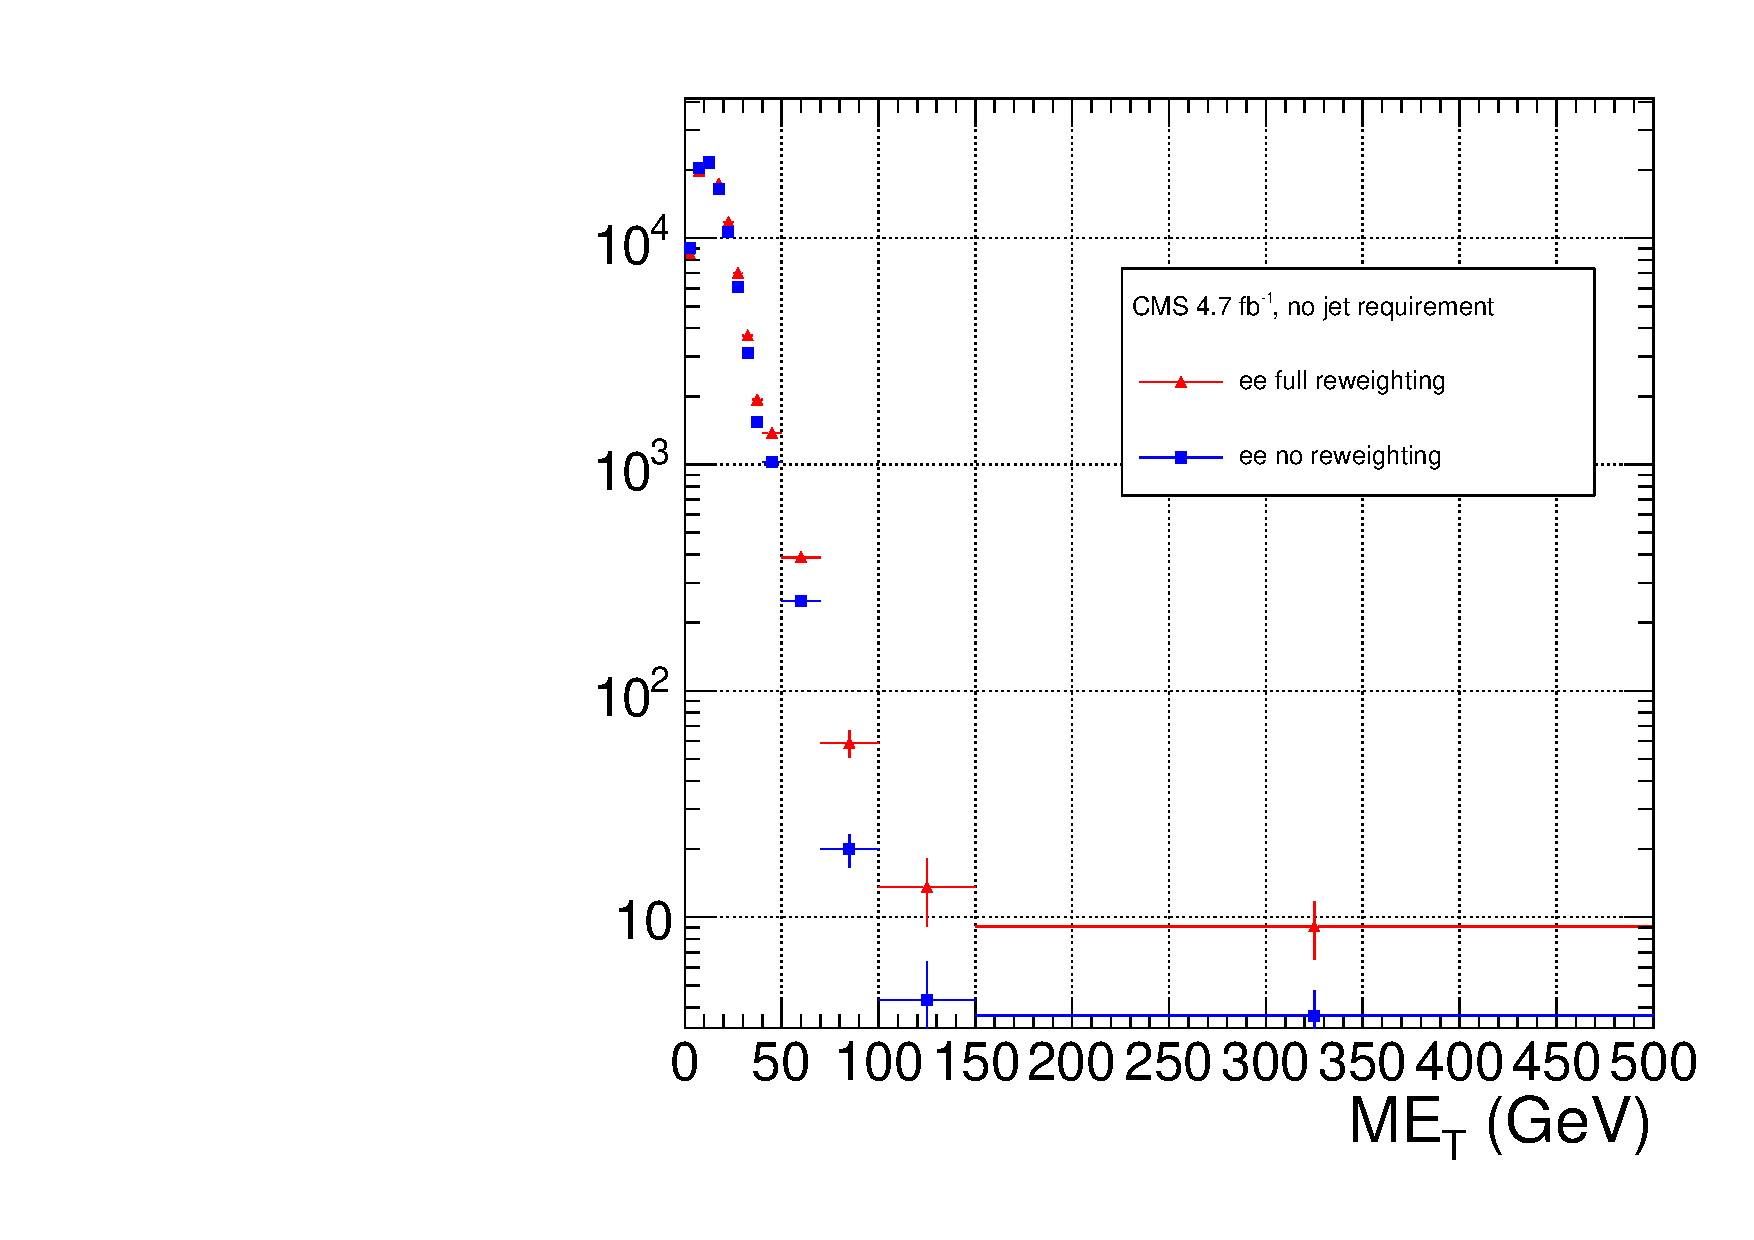
\includegraphics[scale=0.25]{ee_dijet_pT_and_Nj_vs_no_reweighting}}
%	\hspace{1cm}
%	\subfloat[$\mathit{ff}$ \MET spectra.]{\label{fig:ff_dijet_pT_and_Nj_vs_no_reweighting}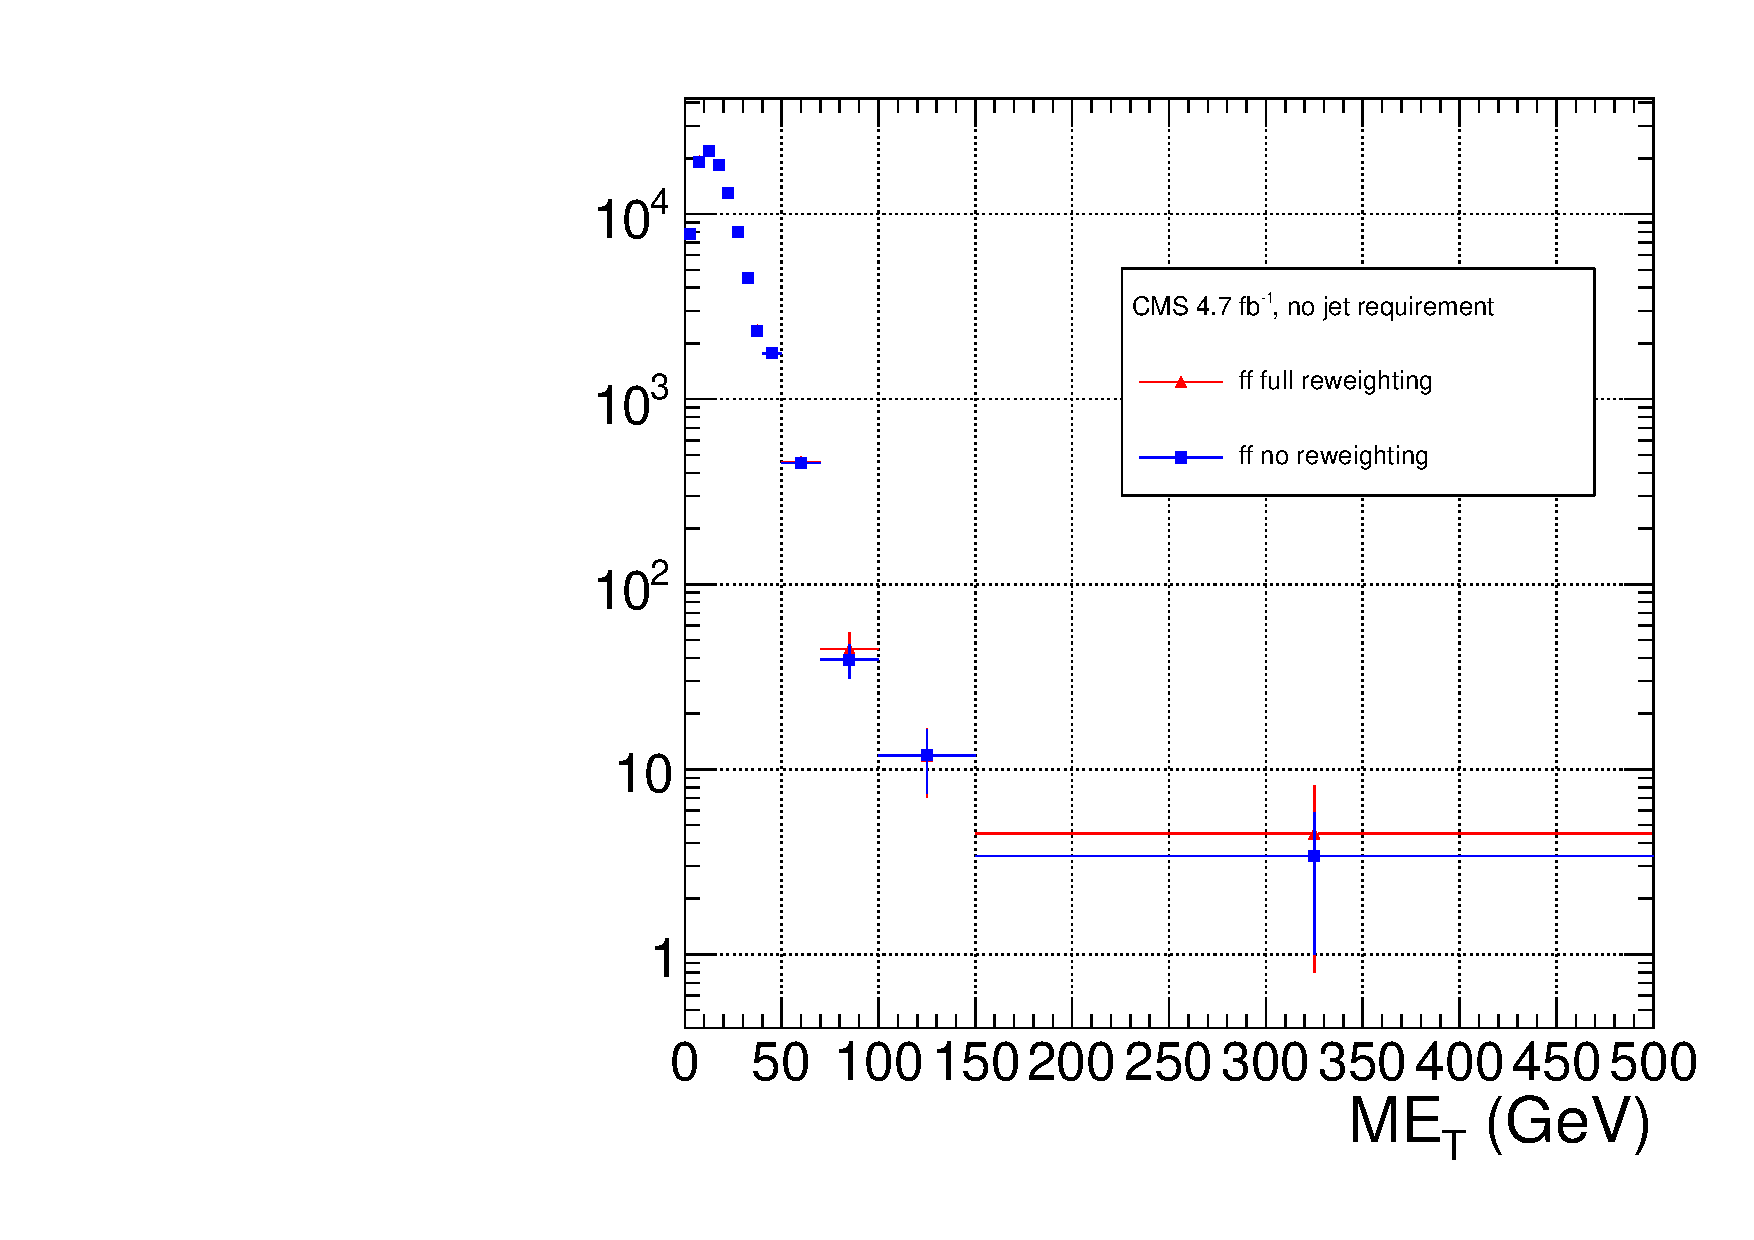
\includegraphics[scale=0.25]{ff_dijet_pT_and_Nj_vs_no_reweighting}}
%	\caption{\MET spectra of the $ee$ and $\mathit{ff}$ control samples.  Squares indicate full di-EM $p_{T}$ + number of jets reweighting; triangles indicate no reweighting.  PF $p_{T}$ (cf. p.~\pageref{fig:ET_bias_vs_EMF}) is used to calculate the di-EM $p_{T}$.  The full normalization procedure is employed, along with $ee$ sideband subtraction (discussed in Sec.~\ref{sec:ee Control Sample}).}
%	\label{fig:reweighting_vs_no_reweighting}
%\end{figure}

\subsection{Normalization}
\label{sec:Normalization}

After reweighting, the \MET distributions of the QCD control samples are normalized to the \MET $< 20$ GeV region of the candidate $\gamma\gamma$ \MET spectrum, where signal contamination is low.  The normalization factor is ($N_{\gamma\gamma}^{\not\!\! E_{T} < 20 \mathrm{GeV}} - N_{\mathrm{electroweak}}^{\not\!\! E_{T} < 20 \mathrm{GeV}})/N_{\mathrm{control}}^{\not\!\! E_{T} < 20 \mathrm{GeV}}$, where $N_{\mathrm{electroweak}}^{\not\!\! E_{T} < 20 \mathrm{GeV}}$ is the expected number of electroweak background events with \MET $< 20$ GeV (discussed in Section~\ref{sec:Modeling the Electroweak Background}).

\subsection{$\mathit{ff}$ Control Sample}
\label{ff Control Sample}

%- for the ee case, explain the sideband subtraction procedure
%	- show the sideband di-EM pT spectra
%	- show the sideband weights
%- show the di-EM pT spectra
%- show the weights
%- show the final MET plot with systematics but say they'll be explained later

%QCD control samples:
%ff
%show upper cut optimization
%show di-EM pT spectra and weights
%ee
%obvious that it's a well-measured EM object
%- for the ee case, explain the sideband subtraction procedure
%	- show the sideband di-EM pT spectra
%	- show the sideband weights
%show di-EM pT spectra and weights

\section{Modeling the Electroweak Background}
\label{sec:Modeling the Electroweak Background}

%EW background
%explain the procedure
%show the ee and eg fits
%show the pT dependence

\section{Systematic Errors}
\label{sec:Systematic Errors}

%systematic studies
%variations in shape of dijet pT spectra and jet bin migration due to statistics and JES
%show that effect of rebinning the dijet pT weights is covered by the 1000-toys procedure
%derive a systematic from subtracting the ee sidebands with different relative weights
%effect of reweighting with and without Nj component
%effect of di-EM vs. dijet pT reweighting
%corrected vs. uncorrected MET
%HT, MHT, Nj ee vs. ff before and after reweighting

%ee as cross-check
%slightly better MET resolution than gg or ff
%MC closure
%agreement in bins of rho
%...

%discuss Dec. vs. Jan. plots in ~/RA3/data--they show that the changes do not significantly affect the result except in the normalization, because of the reduction in gg/eg triggers
%- run with latest dijet pT reweighting and compare to old
%	- changes: added 26/18 trigger, removed R9Id for gg/eg, r9 < 1
%	- result: agreement pretty much the same, fewer overall events


\subsection{Jet Energy Scale Uncertainty}

The dijet \pT reweighting method utilizes jets corrected for imperfect calorimeter response (see Sec.~\ref{sec:Jets and Missing Transverse Energy} for a description of the jet reconstruction and correction procedure).  Since the applied jet energy scale (JES) factor has an error associated to it due to the limitations of the JES derivation (\cite{CMS_JES_paper} and Sec.~\ref{sec:Jets and Missing Transverse Energy}), this uncertainty must be propagated to the uncertainty on the dijet \pT weights.

The JES contribution to the dijet \pT weights is estimated by performing 1000 pseudo-experiments on each of the $\gamma\gamma$ and ff samples.  For the purpose of estimating the JES error, the results of the true experiment may be thought of as a set of measurements:

\begin{itemize}
  \item The set of \textbf{uncorrected jet 4-vectors} corresponding to the \textbf{leading EM object} in the $\gamma\gamma$ sample $\left\{\mbox{p}_{\mbox{j}1}^{\mu1}, \mbox{p}_{\mbox{j}1}^{\mu2},...,\mbox{p}_{\mbox{j}1}^{\mu \mbox{N}_{\gamma\gamma}}\right\}$
  \item The set of \textbf{uncorrected jet 4-vectors} corresponding to the \textbf{trailing EM object} in the $\gamma\gamma$ sample $\left\{\mbox{p}_{\mbox{j}2}^{\mu1}, \mbox{p}_{\mbox{j}2}^{\mu2},...,\mbox{p}_{\mbox{j}2}^{\mu \mbox{N}_{\gamma\gamma}}\right\}$
  \item The set of \textbf{JES} accompanying the uncorrected jet 4-vectors corresponding to the \textbf{leading EM object} in the $\gamma\gamma$ sample $\left\{\mbox{c}_{\mbox{j}1}^{1}, \mbox{c}_{\mbox{j}1}^{2},...,\mbox{c}_{\mbox{j}1}^{\mbox{N}_{\gamma\gamma}}\right\}$
  \item The set of \textbf{JES} accompanying the uncorrected jet 4-vectors corresponding to the \textbf{trailing EM object} in the $\gamma\gamma$ sample $\left\{\mbox{c}_{\mbox{j}2}^{1}, \mbox{c}_{\mbox{j}2}^{2},...,\mbox{c}_{\mbox{j}2}^{\mbox{N}_{\gamma\gamma}}\right\}$
  \item The set of \textbf{JES uncertainties} accompanying the uncorrected jet 4-vectors corresponding to the \textbf{leading EM object} in the $\gamma\gamma$ sample $\left\{\sigma_{\mbox{cj}1}^{1}, \sigma_{\mbox{cj}1}^{2},...,\sigma_{\mbox{cj}1}^{\mbox{N}_{\gamma\gamma}}\right\}$
  \item The set of \textbf{JES uncertainties} accompanying the uncorrected jet 4-vectors corresponding to the \textbf{trailing EM object} in the $\gamma\gamma$ sample $\left\{\sigma_{\mbox{cj}2}^{1}, \sigma_{\mbox{cj}2}^{2},...,\sigma_{\mbox{cj}2}^{\mbox{N}_{\gamma\gamma}}\right\}$
  \item The set of \textbf{uncorrected jet 4-vectors} corresponding to the \textbf{leading EM object} in the ff sample $\left\{\mbox{p}_{\mbox{j}1}^{\mu1}, \mbox{p}_{\mbox{j}1}^{\mu2},...,\mbox{p}_{\mbox{j}1}^{\mu \mbox{N}_{\mbox{ff}}}\right\}$
  \item The set of \textbf{uncorrected jet 4-vectors} corresponding to the \textbf{trailing EM object} in the ff sample $\left\{\mbox{p}_{\mbox{j}2}^{\mu1}, \mbox{p}_{\mbox{j}2}^{\mu2},...,\mbox{p}_{\mbox{j}2}^{\mu \mbox{N}_{\mbox{ff}}}\right\}$
  \item The set of \textbf{JES} accompanying the uncorrected jet 4-vectors corresponding to the \textbf{leading EM object} in the ff sample $\left\{\mbox{c}_{\mbox{j}1}^{1}, \mbox{c}_{\mbox{j}1}^{2},...,\mbox{c}_{\mbox{j}1}^{\mbox{N}_{\mbox{ff}}}\right\}$
  \item The set of \textbf{JES} accompanying the uncorrected jet 4-vectors corresponding to the \textbf{trailing EM object} in the ff sample $\left\{\mbox{c}_{\mbox{j}2}^{1}, \mbox{c}_{\mbox{j}2}^{2},...,\mbox{c}_{\mbox{j}2}^{\mbox{N}_{\mbox{ff}}}\right\}$
  \item The set of \textbf{JES uncertainties} accompanying the uncorrected jet 4-vectors corresponding to the \textbf{leading EM object} in the ff sample $\left\{\sigma_{\mbox{cj}1}^{1}, \sigma_{\mbox{cj}1}^{2},...,\sigma_{\mbox{cj}1}^{\mbox{N}_{\mbox{ff}}}\right\}$
  \item The set of \textbf{JES uncertainties} accompanying the uncorrected jet 4-vectors corresponding to the \textbf{trailing EM object} in the ff sample $\left\{\sigma_{\mbox{cj}2}^{1}, \sigma_{\mbox{cj}2}^{2},...,\sigma_{\mbox{cj}2}^{\mbox{N}_{\mbox{ff}}}\right\}$
\end{itemize}
%
From these measurements, the $\gamma\gamma$ and ff dijet \pT spectra and the resulting ff dijet weights can be calculated.  In each of the 1000 pseudo-experiments, a new set of JES factors is generated according to the measured JES uncertainties, and new dijet \pT spectra and weights are subsequently calculated.  The spread of the 1000 weights (binned in dijet \pT) is taken as the error due to JES uncertainty.  The total error on the weights is the quadrature sum of the JES error and the statistical error, and is propagated to the error on the final \MET measurement via a similar pseudo-experiment procedure described in Sec.~\ref{sec:Statistical Uncertainty in the ff or ee Weights}.\footnote{The \MET is uncorrected and therefore its central value per event is unaffected by a change in the JES.}

%do this check
If the JES uncertainty were to cause the jet energy to be reconstructed below the 20 GeV ntuple cut, there could be a small error or bias in the \MET introduced due to EM-matched jets falling below the matching threshold.  The percentage of jets lost due to jet \ET matching threshold has been checked in data, and found to be X\% (X\% of events).  Furthermore, the trailing EM \ET cut is 25 GeV/c, implying that the JES would have to be mis-measured by at least 20\% to fall below the jet matching threshold.  Since the typical JES uncertainty is no more than 5\%, a mis-measurement of this type is a 4$\sigma$ event and should occur in only 0.1\% of cases.  As expected, this effect is negligible, as shown in Figure X.

%\begin{figure}
%	\centering
%	\subfloat[ff dijet \pT weights including effect of jets falling below the matching threshold.]{\label{fig:dummy}\includegraphics[scale=0.7]{dummy}}
%	\hspace{1cm}
%	\subfloat[ff dijet \pT weights neglecting effect of jets falling below the matching threshold.]{\label{fig:dummy}\includegraphics[scale=0.7]{dummy}}
%	\hspace{1cm}
%	\subfloat[Percentage difference between JES errors shown in (a) and (b).]{\label{fig:dummy}\includegraphics[scale=0.7]{dummy}}
%	\caption{ff dijet \pT weights with JES error.}
%\end{figure}

\subsection{Statistical Uncertainty in the ff or ee Weights}
\label{sec:Statistical Uncertainty in the ff or ee Weights}

\section{Results}
\label{sec:Results}

%results
%final number in signal region with all stat. and syst. errors included
%reminder table of all uncertainties that are described more thoroughly in previous sections
%expectation from GGM models (1 that can be excluded, 1 that can't)

\end{document}